% CVPR 2027 Paper Draft
% Theory of cross-embodiment (ego->robot) data mixing + controlled dual-domain Push-T study
\documentclass[10pt,twocolumn,letterpaper]{article}

%%%%%%%%% PAPER TYPE  - PLEASE UPDATE FOR FINAL VERSION
% \usepackage{cvpr}              % To produce the CAMERA-READY version
\usepackage[review]{cvpr}      % To produce the REVIEW version
% \usepackage[pagenumbers]{cvpr} % To force page numbers, e.g. for an arXiv version

% Import additional packages in the preamble file, before hyperref
%% Preamble: kit defaults + project additions

%% Official support for 2-column teaser figure
\usepackage{cuted} %< for strip environment

%% For auto-referencing of figures
\usepackage{currfile} %< for \currfilebase macro

%% caption support for teaser
\usepackage{caption}

%% Inline annotations
\newcommand{\red}[1]{{\color{red}#1}}
\newcommand{\todo}[1]{{\color{red}#1}}
\newcommand{\TODO}[1]{\textbf{\color{red}[TODO: #1]}}
%% Disable for camera ready / submission by uncommenting these lines:
% \renewcommand{\TODO}[1]{}
% \renewcommand{\todo}[1]{#1}

%% ---------- Project additions ----------
\usepackage{amsmath}
\usepackage{amssymb}
\usepackage{amsthm}
\usepackage{booktabs}
\usepackage{graphicx}
\usepackage{subcaption}
\usepackage{multirow}

\newtheorem{theorem}{Theorem}
\newtheorem{corollary}[theorem]{Corollary}
\newtheorem{lemma}[theorem]{Lemma}
\newtheorem{proposition}[theorem]{Proposition}
\theoremstyle{definition}
\newtheorem{assumption}{Assumption}
\theoremstyle{remark}
\newtheorem{remark}{Remark}

%% Notation macros
\newcommand{\R}{\mathbb{R}}
\newcommand{\E}{\mathbb{E}}
\newcommand{\risk}{\mathcal{R}_T}        % robot-domain excess risk
\newcommand{\riske}{\bar{\mathcal{R}}_T} % deterministic equivalent
\newcommand{\nr}{n_r}
\newcommand{\nh}{n_h}
\newcommand{\kex}{\kappa_{\mathrm{ex}}}  % ego<->teleop exchange rate


\definecolor{cvprblue}{rgb}{0.21,0.49,0.74}
\usepackage[pagebackref,breaklinks,colorlinks,allcolors=cvprblue]{hyperref}

%%%%%%%%% PAPER ID  - PLEASE UPDATE
\def\paperID{*****} % *** Enter the Paper ID here
\def\confName{CVPR}
\def\confYear{2027}

%%%%%%%%% TITLE
\title{When Does Egocentric Human Data Help Robot Policies?\\
A Spectral Theory of Cross-Embodiment Data Mixing}

%%%%%%%%% AUTHORS (review version: anonymized)
\author{Anonymous \confName~\confYear~submission\\
Paper ID \paperID\\
{\tt\small https://anonymous.4open.science/ (code and data to be released)}
}

\begin{document}
\maketitle
\begin{figure*}[t]
  \centering
  \begin{subfigure}[t]{0.24\linewidth}
    \centering
    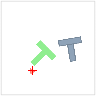
\includegraphics[width=\linewidth]{fig/render_robot.png}
    \caption{Robot domain (target)}
    \label{fig:teaser-robot}
  \end{subfigure}
  \hfill
  \begin{subfigure}[t]{0.24\linewidth}
    \centering
    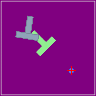
\includegraphics[width=\linewidth]{fig/render_human.png}
    \caption{Surrogate ego domain (source)}
    \label{fig:teaser-human}
  \end{subfigure}
  \hfill
  \begin{subfigure}[t]{0.47\linewidth}
    \centering
    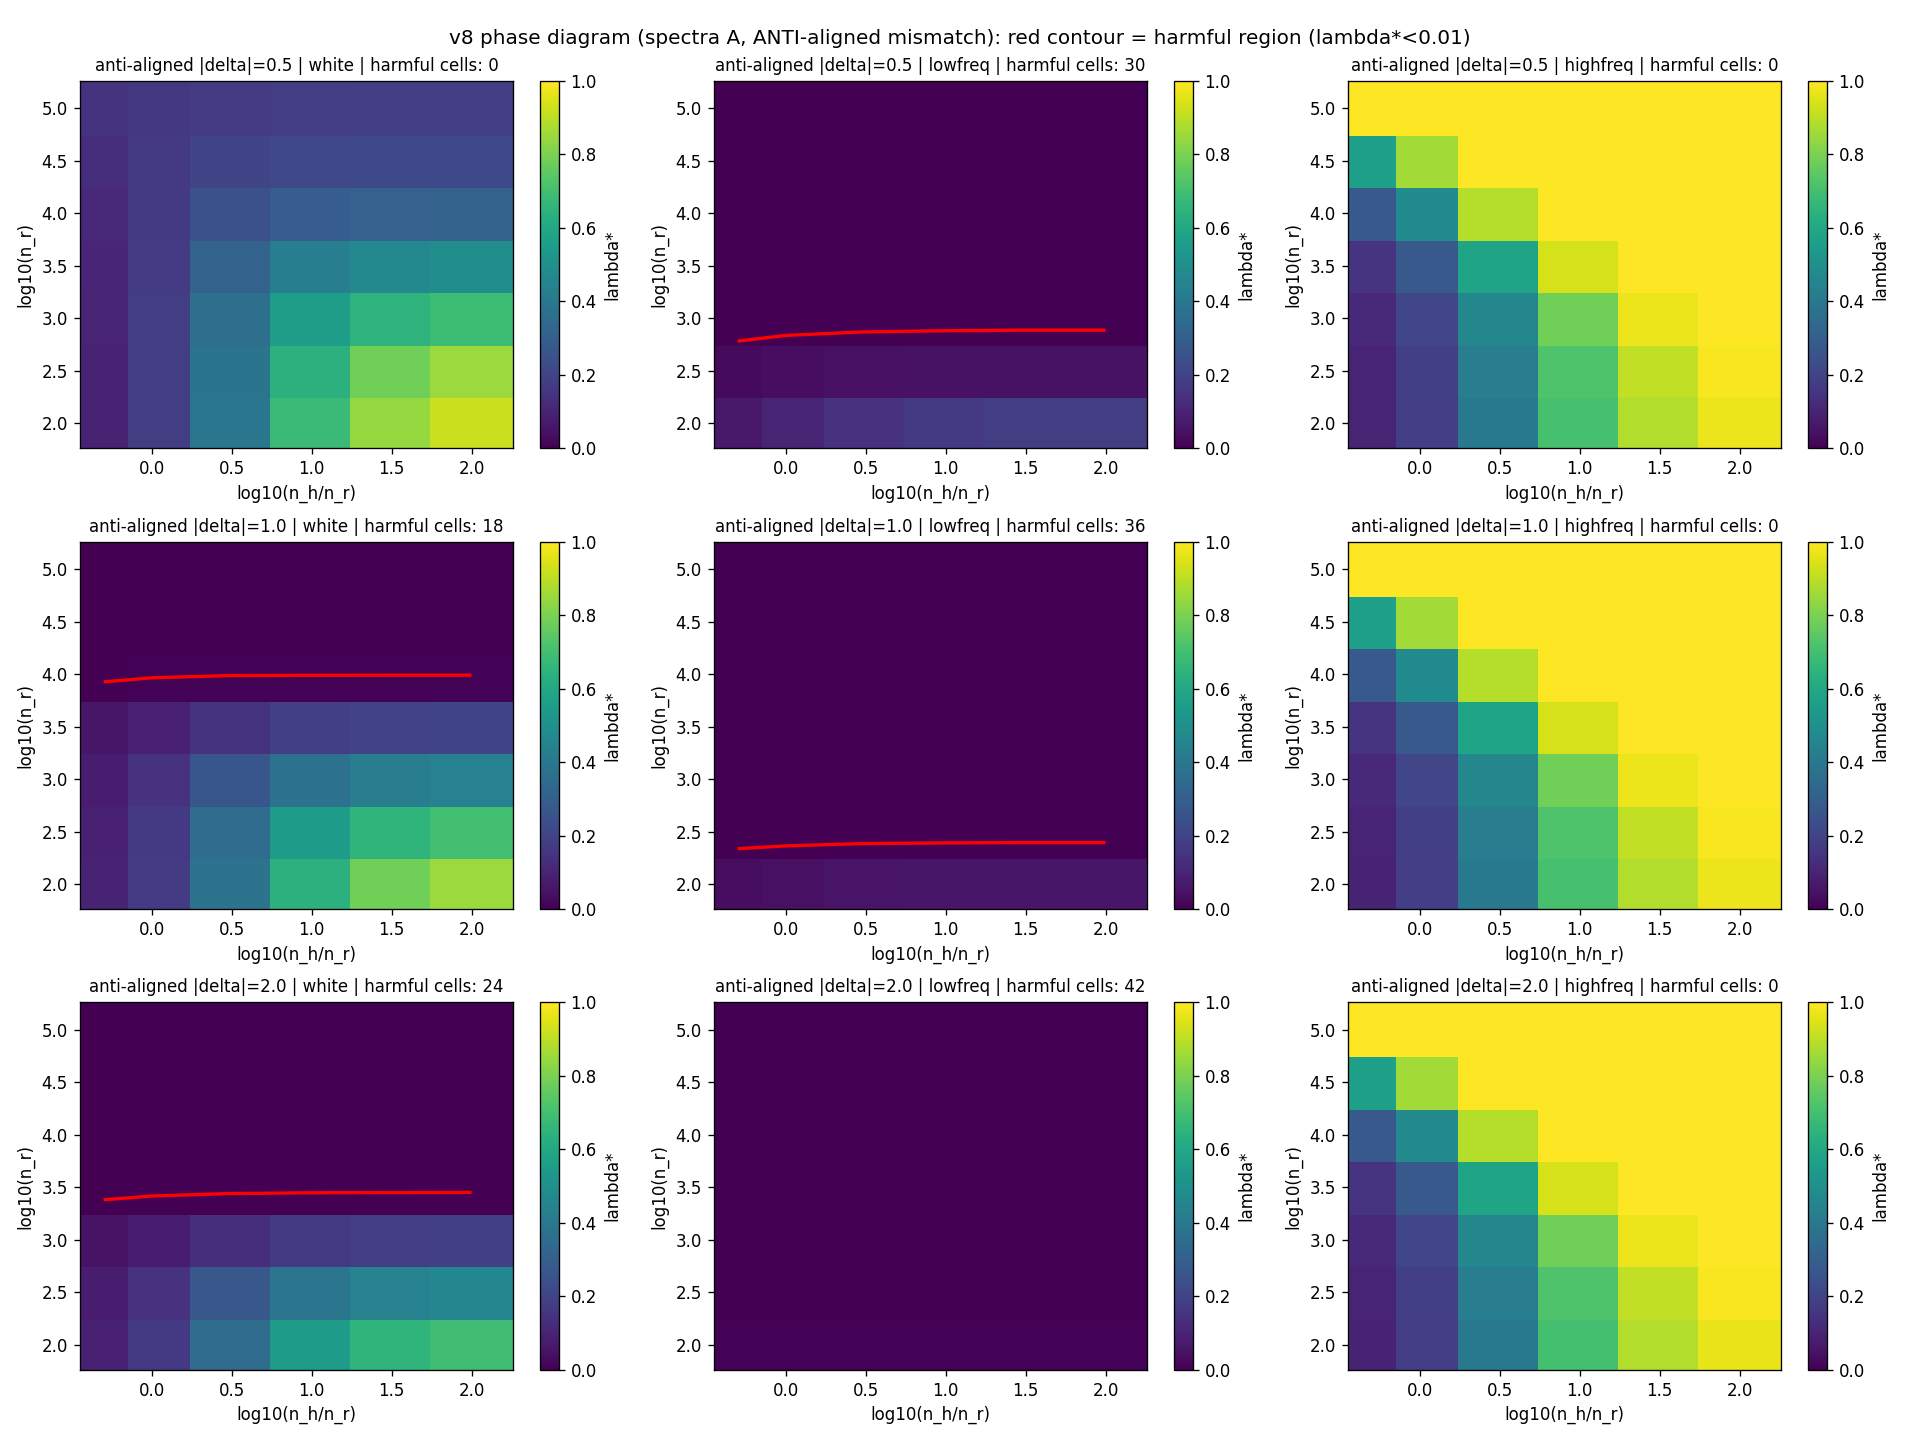
\includegraphics[width=\linewidth]{fig/phase_v8_anti.png}
    \caption{Theory: where mixing hurts}
    \label{fig:teaser-phase}
  \end{subfigure}
  \caption{\textbf{Cross-embodiment data mixing, modeled.}
  (a,b)~Our controlled dual-domain Push-T testbed pairs a robot domain with a surrogate egocentric-human domain that differs in appearance, actuator, friction, and task geometry (mirrored T-block configurations).
  (c)~The theory predicts \emph{where mixing hurts}: optimal mixing ratio $\lambda^*$ over the $(\nr,\, \nh/\nr)$ plane under anti-aligned mismatch; low-frequency-concentrated mismatch collapses $\lambda^*\!\to\!0$ (dark region), while the same mismatch energy placed on high-frequency coordinates is harmless everywhere (Sec.~\ref{sec:theory}).}
  \label{fig:teaser}
\end{figure*}

\begin{abstract}
Robot demonstration data is expensive to collect; egocentric human data is cheap and abundant.
Mixing the two is increasingly common in practice, yet the design rules are empirical folklore: reported substitution ratios of 4--5 ego-hours per teleoperation-hour, occasional negative transfer, and no principled answer to \emph{when} and \emph{how much} egocentric data helps a robot policy.
We give a first-principles account. We model the two domains as Gaussian covariates with power-law feature spectra, the embodiment gap as a task-vector mismatch decomposed in the shared spectral basis, and the policy fit as mixture-weighted ridge regression evaluated on robot-domain risk.
Our main theorem characterizes the mixture risk in closed per-coordinate form (Monte-Carlo verified to 1--2\% relative error) and reveals a three-term structure of the marginal benefit of human data: an alignment term, a variance-reduction term, and a spectral-coverage term.
From it we derive an exact phase-transition criterion: mixing is beneficial at all robot sample sizes iff a functional $H$ of the mismatch spectrum and the spectra is non-positive; otherwise a critical robot sample size $\nr^{\mathrm{crit}} = K/H$ appears beyond which human data should be discarded --- recovering the classical source-discard transition as regularization vanishes.
An exchange-rate corollary defines $\kex$, the number of robot demonstrations equivalent to one egocentric demonstration, shows it is increasing in the inter-domain spectral gap and capped at $1$, and lands in the same range as empirically reported substitution ratios.
We validate the structural predictions in a controlled dual-domain Push-T testbed with diffusion policies: the first batch confirms the predicted non-monotone benefit with an interior optimum (up to $+32\%$ closed-loop coverage) and harm boundary, shows the benefit grows with training budget and that alignment strength is itself non-monotone, and surfaces an open-loop/closed-loop divergence as a target for the next theory iteration.
\end{abstract}

\section{Introduction}
\label{sec:intro}

Robot learning is data-hungry, and its current fuel --- teleoperated robot demonstrations --- is expensive, slow to collect, and hard to scale.
Egocentric human data offers a tempting substitute: wearable-camera recordings of humans performing manipulation tasks are cheap, abundant, and semantically aligned with the tasks we want robots to do.
A growing line of systems therefore mixes egocentric human data into robot policy training, using hand-mounted grippers~\cite{kareer2024egomimic}, hand-held interfaces~\cite{chi2024universal}, portable motion-capture rigs~\cite{wang2024dexcap}, or simulation surrogates of the human embodiment~\cite{egobridge2025}, and reports substantial gains.

Yet the practice is ahead of the principle. Reported pipelines rely on rules of thumb --- fixed mixing ratios, substitution rates on the order of 4--5 ego-hours per teleoperation-hour~\cite{zevaego2025}, alignment losses tuned by trial and error --- and the same recipe that helps in one setting degrades the policy in another through negative transfer and gradient conflict.
Classical domain-adaptation theory~\cite{bendavid2010theory,zhao2019learning} explains \emph{why} source data can help or hurt, but its bounds are existential rather than operational: they do not tell a practitioner what the optimal mixing ratio is, when mixing is strictly harmful, or what one egocentric demonstration is worth in units of robot demonstrations.

This paper takes a step toward such an operational theory, and validates it in a controlled testbed.
We abstract cross-embodiment data mixing into a \emph{dual-domain model}: observations in each domain are Gaussian covariates with power-law feature spectra $\lambda^e_j \asymp j^{-\alpha_e}$ --- motivated by the heavy-tailed spectra ubiquitously observed in learned visual representations~\cite{martin2021implicit} --- the two domains share a spectral basis, and the embodiment gap is decomposed into a task mismatch vector $\delta$, an alignment coefficient $c = \delta^\top\beta^*$, and per-domain noise.
Policies are fit by mixture-weighted ridge regression and evaluated by excess risk on the robot domain.
The model is deliberately simple --- linear labels, ridge estimation --- because its role is to supply \emph{falsifiable structural predictions} (signs, phase boundaries, monotone directions), which we then test on a diffusion policy in a controlled dual-domain Push-T environment rather than to numerically match a deep learner.

Our findings are fourfold.
First, the mixture risk admits a closed per-coordinate characterization (Theorem~\ref{thm:t1a}), exact up to a relative error of $O(n_r^{-3/2})$ and verified numerically to 1--2\%; the analysis exposes a \emph{label-feedthrough} effect in which out-of-coordinate signal energy acts as effective noise, $\tilde\sigma_e^2 = \sigma_e^2 + F_e$, which is essential for quantitative accuracy.
Second, the marginal benefit of human data decomposes into three interpretable terms --- alignment, variance reduction, and spectral coverage --- whose competition yields an exact phase-transition criterion (Theorem~\ref{thm:h}): mixing is marginally beneficial at \emph{all} robot sample sizes iff $H \le 0$ for an explicit functional $H$; otherwise a critical threshold $\nr^{\mathrm{crit}} = K/H$ appears, and the classical discard-the-source transition~\cite{bendavid2010theory} is recovered exactly as regularization vanishes.
Strikingly, whether mixing hurts is governed less by the \emph{magnitude} of the mismatch than by the \emph{location of its spectrum} relative to the risk-weighting spectrum: mismatch concentrated on low-frequency, high-risk-weight coordinates is harmful almost everywhere, while the same energy on high-frequency coordinates is harmless (Fig.~\ref{fig:teaser}).
Third, an exchange-rate corollary (Corollary~\ref{cor:kex}) defines $\kex$, the number of robot demonstrations equivalent to one egocentric demonstration, and shows it increases with the spectral gap $\alpha_r - \alpha_h$, decreases with mismatch and with $\nr$, and is capped at $1$ --- beyond which human data covers directions that no amount of additional robot data reaches.
The predicted range $\kex \approx 0.2$--$0.6$ in the small-gap regime quantitatively matches empirically reported 4--5:1 substitution ratios~\cite{zevaego2025}.
Fourth, we build a controlled dual-domain Push-T testbed (Sec.~\ref{sec:platform}) in which every gap component (appearance, actuator, friction, task geometry, coverage) is independently manipulable, and run a first batch of mixture experiments with a diffusion policy (Sec.~\ref{sec:experiments}).
The experiments confirm the theory's three headline structural predictions: naive mixing yields a \emph{non-monotone} benefit curve with an interior optimum ($\lambda^* \approx 0.5$, $+28\%$ closed-loop coverage) and a harm boundary at $\lambda \to 1$; the benefit \emph{grows} with training budget ($+32\%$ at 150 epochs, relieving overfitting exactly as the variance term predicts); and alignment strength is itself non-monotone --- light MMD alignment helps while strong alignment hurts at intermediate $\lambda$, consistent with the coverage term's logic.
They also surface a sharp open-loop/closed-loop divergence: open-loop robot-domain prediction error keeps improving well past the closed-loop optimum, evidence that prediction and execution must be bridged explicitly.
The optimum's quantitative position (predicted $\lambda^* \approx 0.12$ vs.\ measured $\approx 0.5$) is off, and we state the gap and its sources plainly.

\paragraph{Contributions.}
(i)~A dual-domain spectral model of cross-embodiment data mixing with an explicit mismatch decomposition (Sec.~\ref{sec:setup}).
(ii)~A closed-form risk characterization of the mixture estimator with provable error control, verified to 1--2\% (Sec.~\ref{sec:theory}, Theorem~\ref{thm:t1a}).
(iii)~An exact phase-transition criterion for harmful mixing (Theorem~\ref{thm:h}) and an exchange-rate corollary (Corollary~\ref{cor:kex}) that explains empirical substitution ratios.
(iv)~A controlled dual-domain Push-T testbed and a first experimental batch testing the theory's structural predictions with diffusion policies (Secs.~\ref{sec:platform}--\ref{sec:experiments}).
Proofs, numerical verification protocols, and experimental details are in the supplementary material.

\section{Related work}
\label{sec:related}

\paragraph{Egocentric human data for robot learning.}
Egocentric video has long served as a representation prior: Ego4D~\cite{grauman2022ego4d} supplies large-scale first-person video, and R3M/VIP-style pretraining~\cite{nair2022r3m,ma2022vip} distills it into visual features for downstream control.
A more recent line injects egocentric data \emph{directly into policy training}: EgoMimic~\cite{kareer2024egomimic} uses hand-mounted grippers whose kinematics match the robot, UMI~\cite{chi2024universal} uses hand-held grippers with visual-inertial pose recovery, DexCap~\cite{wang2024dexcap} uses portable mocap, and EgoBridge~\cite{egobridge2025} studies mixing in simulation with explicit domain gaps.
Cross-embodiment robot corpora~\cite{openx2024} face a cousin of the same problem across robot morphologies.
These works establish that mixing \emph{can} help and document substitution ratios~\cite{zevaego2025} and failure modes, but stop short of a principled account of when and why --- the gap this paper addresses.

\paragraph{Domain adaptation and mixture theory.}
Classical domain-adaptation theory bounds target error by source error plus a discrepancy and a shared-optimal-hypothesis term~\cite{bendavid2010theory}; later work asks when quantity compensates for quality~\cite{bendavid2014quantity}, characterizes the value of target data via transfer exponents~\cite{hanneke2019value}, and shows that enforced representation invariance can provably \emph{hurt} when label marginals differ~\cite{zhao2019learning}.
On the practice side, data-mixture scaling laws~\cite{wu2026mixture} and analyses of sim-real co-training~\cite{lei2026simreal} give empirical-fit models of multi-source learning.
Closest to us is the ridge-regression scaling analysis of~\cite{wu2026mixture}, whose minimax characterization assumes matched task vectors across domains; our model adds an explicit mismatch spectrum, which is precisely the object that governs harmful mixing (Theorem~\ref{thm:h}).
Relative to all of the above, our contribution is an \emph{operational} theory: closed-form mixture risk, an explicit critical-threshold formula, and an exchange rate, all stated in quantities estimable from data.

\paragraph{Technical tools.}
Our analysis builds on the ridge-regression literature under power-law spectra~\cite{dobriban2018high,hastie2022surprises}, with two differences that matter: the robot-domain risk is $\Sigma_r$-weighted (only target-geometry errors count), and the sample-level coupling between coordinates induces a \emph{label-feedthrough} term that acts as effective noise (Sec.~\ref{sec:setup}).
On the alignment side we use kernel MMD~\cite{gretton2012kernel,long2015learning} as the alignment-strength knob in experiments; gradient-conflict diagnostics follow the multi-task learning literature~\cite{yu2020surgery}; and the impossibility caveats of invariant-representation approaches~\cite{zhao2019learning,arjovsky2019invariant} inform our negative results.

\section{A dual-domain model of cross-embodiment mixing}
\label{sec:setup}

We abstract the problem to its statistical skeleton.
Two domains provide training data: the \emph{robot domain} $r$ (target; teleoperated demonstrations) and the \emph{human domain} $h$ (source; egocentric recordings).
We write $e \in \{r,h\}$ for the domain index.

\begin{assumption}[Data model]\label{ass:a1}
Coordinates $j = 1,\dots,p$ index a shared spectral basis.
Observations are $x_e = \Sigma_e^{1/2} u_e$ with $u_e$ standard Gaussian and $\Sigma_e = \mathrm{diag}(\lambda^e_j)$ diagonal with power-law spectra
\begin{equation}
  \lambda^e_j \asymp j^{-\alpha_e}, \qquad \lambda^e_1 = 1,
  \label{eq:powerlaw}
\end{equation}
and throughout we abbreviate $a_j = \lambda^r_j$, $b_j = \lambda^h_j$.
\end{assumption}

\begin{assumption}[Labels and mismatch]\label{ass:a2}
$y_r = \langle \beta^*, x_r \rangle + \varepsilon_r$ in the robot domain; $y_h = \langle \beta^* + \delta, x_h \rangle + \varepsilon_h$ in the human domain.
The \emph{task mismatch} $\delta$ absorbs retargeting error, kinematic differences, and residual appearance-induced shifts; its \emph{alignment} with the task is $c = \delta^\top\beta^*$.
Noise variances are $\sigma_e^2$, and $\beta^*$ obeys an ellipsoid constraint $\sum_j j^{2s}\beta_j^{*2} \le 1$ with $s > 0$.
\end{assumption}

\begin{assumption}[Mixture estimator]\label{ass:a3}
Given $\nr$ robot and $\nh$ human samples and a mixing ratio $\lambda \in [0,1]$, per-sample weights are $w_r = (1-\lambda)/\nr$, $w_h = \lambda/\nh$.
We analyze the \emph{diagonalized ridge} estimator
\begin{equation}
  \hat\beta_j = \frac{w_r T_{rj} + w_h T_{hj}}{w_r S_{rj} + w_h S_{hj} + \mu},
  \qquad \mu > 0,
  \label{eq:estimator}
\end{equation}
with $S_{ej} = \|X_{e,:j}\|^2$, $T_{ej} = X_{e,:j}^\top y_e$; $\mu$ is the ridge penalty and stands in for explicit or implicit regularization (weight decay, early stopping).
\end{assumption}

The evaluation criterion is the \emph{robot-domain excess risk}, weighted by the robot geometry:
\begin{equation}
  \risk(\lambda) = \E\big\| \hat\beta(\lambda) - \beta^* \big\|^2_{\Sigma_r}.
  \label{eq:risk}
\end{equation}
Only errors in directions the robot actually visits are penalized --- this weighting turns out to be essential for the phase structure in Sec.~\ref{sec:theory}.

\paragraph{Label feedthrough.}
A subtle point drives the quantitative accuracy of the theory.
Although the population covariances are diagonal, the \emph{sample} Gram matrices are not: the label projection $T_{ej}$ picks up contributions from all other coordinates, $T_{ej} = S_{ejj}\beta_{e,j} + \sum_{k\neq j} S_{ejk}\beta_{e,k} + X_{e,:j}^\top\varepsilon_e$.
The middle term is mean-zero with variance $\nr\lambda^e_j F_e$ (and similarly for $h$), where $F_e = \sum_k \lambda^e_k\beta_{e,k}^2$ is the domain's total signal energy.
Out-of-coordinate signal is therefore indistinguishable from noise, giving rise to the \emph{effective noise}
\begin{equation}
  \tilde\sigma_e^2 = \sigma_e^2 + F_e .
  \label{eq:feedthrough}
\end{equation}
A heavier-tailed human spectrum (small $\alpha_h$) inflates $F_h$: broad coverage carries a hidden per-coordinate SNR cost, which competes with its coverage benefit --- this tension is the microscopic origin of the phase diagrams in Sec.~\ref{sec:theory}.

\paragraph{What the model keeps and discards.}
The model retains the three gap components that mixture practice manipulates --- spectra (coverage), mismatch $\delta$ (embodiment/retargeting), and noise --- and discards the rest (nonlinear observation maps, temporal structure, closed-loop compounding).
Sec.~\ref{sec:experiments} therefore tests only \emph{structural} predictions: signs, monotone directions, and phase-region membership, not pointwise numerical values.
The diagonalization in Assumption~\ref{ass:a3} is a controlled approximation of the full ridge solution; we quantify its gap (8--28\% on the weighted risk) in the supplementary and prove the full-ridge deterministic equivalent there in the fixed-dimension regime.

\section{Theory}
\label{sec:theory}

All proofs and the full numerical-verification protocol are deferred to the supplementary; here we state results and give intuition.

\subsection{Closed-form risk of the mixture estimator}

\begin{theorem}[Risk characterization, T1-a]\label{thm:t1a}
Under Assumptions~\ref{ass:a1}--\ref{ass:a3}, with $\nr,\nh \to \infty$ at fixed ratio $\rho = \nh/\nr$ and $p$ fixed or growing polynomially, with high probability,
\begin{equation}
  \big|\, \risk(\lambda) - \riske(\lambda) \,\big|
  \;\le\; C\big(\kappa_0^{-3} + \nr^{-3/2}\big)\, \riske(\lambda),
  \label{eq:t1a-error}
\end{equation}
where the deterministic equivalent is
\begin{align}
  \riske(\lambda) = \sum_{j > m} a_j\beta_j^{*2} + \sum_{j \le m} a_j\, \mathrm{MSE}^{\det}_j(\lambda),
  \label{eq:t1a}
\end{align}
with per-coordinate closed form
\begin{align}
  \mathrm{MSE}^{\det}_j = \underbrace{\frac{(1{-}\lambda)^2 \tilde\sigma_r^2 a_j / \nr + \lambda^2 \tilde\sigma_h^2 b_j / \nh}{D_j^2}}_{\text{effective variance}}
  + \underbrace{\Big(\frac{\lambda\, b_j \delta_j - \mu \beta^*_j}{D_j}\Big)^2}_{\text{bias square}},
  \label{eq:mse}
\end{align}
where the bias square expands into mismatch energy, shrinkage energy, and an \emph{alignment cross term} $-2\lambda\mu b_j \delta_j \beta^*_j / D_j^2$ whose sign tracks the alignment $c$;
$D_j = (1-\lambda) a_j + \lambda b_j + \mu$, $\tilde\sigma_e^2 = \sigma_e^2 + F_e$ the feedthrough-corrected effective noise of Eq.~\eqref{eq:feedthrough}, and $m$ a self-consistent truncation $m = \max\{j : D_j \ge \kappa_0 \eta_j\}$ with $\eta_j$ the fluctuation scale of the empirical denominator.
Second-order fluctuation corrections to Eq.~\eqref{eq:mse} are derived in the supplementary and included in all numerical evaluations.
\end{theorem}

\paragraph{Proof sketch.}
The chain is elementary once the feedthrough is identified: (i)~a per-coordinate representation of the estimator including the feedthrough term (Lemma~L1); (ii)~exact conditional MSE given the design (Lemma~L2); (iii)~a deterministic equivalent via $\chi^2$ concentration of $S_{ejj}$ and a second-order delta method, in which the only third-order mixed moment closes in the exact form $8\lambda^3 b_j^3\delta_j^2/\nh^2$ (Lemma~L3); (iv)~assembly with a truncation at the information-poor coordinates, where a boundary-band argument keeps the aggregate relative error at $O(\kappa_0^{-3})$ (Lemma~L4).
Every step is scalar random-matrix-free analysis; no new asymptotic-equivalence lemma is needed in the diagonal setting.

\paragraph{Numerical verification.}
Across spectral families and mixing ratios, Eq.~\eqref{eq:mse} matches Monte-Carlo estimates with binned median relative error 0.6--1.6\% and aggregate error $\le 2\%$ (200 replicates, $\sim$200k coordinate-replicates; the supplementary material).
Against the \emph{full} (non-diagonalized) ridge estimator, Eq.~\eqref{eq:t1a} is a variance upper bound; the gap on the weighted risk is 8--28\% depending on the spectral family, and the full-ridge extension (T1-b) is proved in the supplementary for the fixed-dimension regime.

\subsection{When does marginal mixing help? Three forces}

\begin{corollary}[Marginal-benefit decomposition, C1]\label{cor:c1}
The right derivative $\riske'(0^+) = \sum_j a_j\, \partial_\lambda \mathrm{MSE}^{\det}_j(0)$ decomposes per coordinate as (sign flipped so that positive means beneficial)
\begin{align}
  \mathrm{benefit}_j \;\propto\;
  \underbrace{\mu \beta^*_j b_j \delta_j}_{\text{A: alignment}}
  + \underbrace{V_j D_{0j}}_{\text{B: variance}}
  + \underbrace{(V_j + \mu^2\beta_j^{*2})(b_j - a_j)}_{\text{C: coverage}},
  \label{eq:c1}
\end{align}
with $V_j = \tilde\sigma_r^2 a_j / \nr$ and $D_{0j} = a_j + \mu$.
\end{corollary}

The three terms have distinct physical carriers.
A~(alignment) exists only through $\mu$: regularization is what couples the mismatch to the task direction --- with sign set by $c = \delta^\top\beta^*$.
B~(variance) is always positive and vanishes as $\nr$ grows: diminishing returns.
C~(coverage) is positive exactly where the human spectrum is heavier than the robot spectrum, $b_j > a_j$; it is the spectral fingerprint of "the human data sees directions the robot data cannot".
In the unregularized limit only B survives:
\begin{equation}
  \riske'(0^+)\big|_{\mu=0} = -\frac{2\tilde\sigma_r^2}{\nr}\sum_j j^{\alpha_r - \alpha_h} < 0
  \quad\text{always},
  \label{eq:mu0}
\end{equation}
so under-regularized mixture is always beneficial, with magnitude growing in the spectral gap --- the classical picture.

\subsection{The phase transition: an exact criterion}

\begin{theorem}[Harmful-mixing criterion, C2]\label{thm:h}
Define the asymptotic marginal-harm functional (the $\nr\to\infty$, $\nh/\nr$ fixed part of $\riske'(0^+)$ after term B vanishes), for anti-aligned mismatch:
\begin{align}
  H \;=\; \underbrace{2\mu \sum_j \frac{a_j \beta^*_j b_j |\delta_j|}{D_{0j}^2}}_{A_\infty:\ \text{mismatch harm}}
  \;-\; \underbrace{2\mu^2 \sum_j \frac{a_j \beta_j^{*2} (b_j - a_j)}{D_{0j}^3}}_{C_\infty:\ \text{coverage benefit}} .
  \label{eq:h}
\end{align}
Then (i)~$H \le 0$ implies marginal mixing is beneficial at \emph{all} robot sample sizes;
(ii)~$H > 0$ implies a critical robot sample size
\begin{equation}
  \nr^{\mathrm{crit}} = K / H,
  \qquad
  K = 2\tilde\sigma_r^2\,(S_1 + S_2),
  \label{eq:ncrit}
\end{equation}
with $S_1 = \sum_j a_j^2/D_{0j}^2$, $S_2 = \sum_j a_j^2(b_j - a_j)/D_{0j}^3$, beyond which marginal mixing hurts.
\end{theorem}

\paragraph{Exactness.}
The criterion is not an asymptotic slogan.
Numerically (the supplementary material): the predicted mismatch threshold $\|\delta\|^* = 0.674$ (the root of $H$) coincides with the Monte-Carlo phase boundary to within the search resolution, and $\nr^{\mathrm{crit}} \cdot H = 25.866$ is constant across three decades of mismatch magnitude --- the inverse proportionality in Eq.~\eqref{eq:ncrit} is exact.

\paragraph{Two consequences.}
First, \emph{mismatch location beats mismatch magnitude}: because $A_\infty$ weights $|\delta_j|$ by the risk weight $a_j\beta^*_j b_j/D_{0j}^2$, mismatch concentrated on low-frequency, high-risk-weight coordinates is harmful across nearly the whole $(\nr, \nh/\nr)$ plane (42/42 cells at $\|\delta\|=2$), while the same energy on high-frequency coordinates is harmless everywhere (0/42) --- see Fig.~\ref{fig:teaser-phase} and Table~\ref{tab:harmful}.
Second, \emph{$\mu$ is the carrier of the classical transition}: as $\mu \to 0$, $C_\infty \to 0$ and $H = A_\infty > 0$ whenever $c<0$, recovering the discard-the-source transition of classical domain adaptation; at $\mu > 0$ the large-$\nr$ limit of the mixing benefit is $-C_\infty < 0$ --- broad human coverage keeps paying even with abundant robot data.

\begin{table}[t]
  \centering
  \small
  \caption{Harmful-mixing cells (out of 42 grid points of $(\nr, \nh/\nr)$) under anti-aligned mismatch, by mismatch magnitude and \emph{spectral location}.
  Location --- not magnitude --- is the dominant factor; theory: Eq.~\eqref{eq:h}.}
  \label{tab:harmful}
  \begin{tabular}{lccc}
    \toprule
    $\|\delta\|$ & white & low-freq & high-freq \\
    \midrule
    0.5 & 0/42 & 30/42 & 0/42 \\
    1.0 & 18/42 & 36/42 & 0/42 \\
    2.0 & 24/42 & 42/42 & 0/42 \\
    \bottomrule
  \end{tabular}
\end{table}

\subsection{The exchange rate of egocentric data}

\begin{corollary}[Exchange rate, T2]\label{cor:kex}
Define the ego$\leftrightarrow$teleop exchange rate $\kex$ by
\begin{equation}
  \riske(\lambda^*;\, \nr, \nh) = \riske\big(0;\, \nr + \kex\, \nh\big),
  \label{eq:kex}
\end{equation}
\ie, the amount of extra robot data that reproduces the optimal mixture's risk.
Then $\kex$ is (i)~increasing in the spectral gap $\alpha_r - \alpha_h$; (ii)~decreasing in the effective mismatch; (iii)~decreasing in $\nr$; and (iv)~capped: there is a large-gap regime in which $\kex \ge 1$, \ie, human data supplies coverage that \emph{no} amount of additional robot data reproduces.
\end{corollary}

Numerically (Fig.~in suppl.): at zero spectral gap with moderate mismatch and noisier human labels, $\kex \approx 0.42$--$0.59$ --- one ego sample is worth about half a robot sample, the price of the gap; the cap $\kex = 1$ binds from $\alpha_r - \alpha_h \approx 0.5$--$0.75$ upward.
The empirical substitution ratio of 4--5:1 reported for egocentric pipelines~\cite{zevaego2025} corresponds to $\kex \approx 0.2$--$0.25$ and falls inside the predicted small-gap range $0.19$--$0.56$; we note the units caveat (theory prices samples; empirics price hours).
Corollary~\ref{cor:kex} thus turns a practitioner rule of thumb into a computable function of measurable quantities: two spectra, a mismatch spectrum, and noise levels.

\paragraph{The $\nh$ axis: an exact dosage law.}
The classical small-source threshold has a smooth refinement in this model (supplementary material).
At matched spectra the optimal gain is exactly hyperbolic in the human sample size, $g(\nh) = A_1^2/(4A_2(\nh))$ with $A_2(\nh) = A_2^r + B/\nh$; this yields an explicit worth-mixing threshold $\nh^\varepsilon$, a ratio $\lambda^*(\nh)$ growing linearly from zero, and a closed-form exchange rate whose pole is exactly the cap regime of Corollary~\ref{cor:kex}(iv).
Unlike the $\nr$ axis --- a true sign-change transition (Theorem~\ref{thm:h}) --- the $\nh$ axis carries no sign change: once mixing helps at all, it helps at every sample size, and the hard classical threshold is recovered only as the divergence $\nh^\varepsilon \to \infty$.

\section{A controlled dual-domain Push-T testbed}
\label{sec:platform}

Testing the theory requires a testbed in which every component of the embodiment gap is independently manipulable --- something real egocentric datasets do not allow.
We therefore build a \emph{dual-domain} variant of Push-T, following the simulation-side design of EgoBridge~\cite{egobridge2025} with three deliberate deviations (stated below), on top of the diffusion-policy codebase of~\cite{chi2023diffusion}.

\paragraph{Domain construction.}
Both domains share the Push-T task (push a T-shaped block to a goal pose with a point-mass pusher, image observations) and differ along four axes, summarized in Table~\ref{tab:domains} and Fig.~\ref{fig:teaser}: the pusher embodiment (triangle vs.\ circle), the appearance (white vs.\ purple background), the contact dynamics (friction scaled $\times 0.7$ vs.\ unchanged), and the task geometry (the T-block's initial and goal poses are mirrored about the vertical axis in the human domain, so that optimal pushing actions are \emph{not} directly transferable --- a controlled kinematic gap).
The four axes map onto the model's quantities: appearance/friction differences reshape the two spectra $(a_j, b_j)$; the mirrored geometry induces the task mismatch $\delta$; the pusher change alters both.

\begin{table}[t]
  \centering
  \small
  \caption{Dual-domain Push-T construction. The robot domain is the training+evaluation target; the human domain is the mixture source (a \emph{surrogate} for egocentric data, in the spirit of~\cite{egobridge2025}).}
  \label{tab:domains}
  \begin{tabular}{lcc}
    \toprule
     & robot (target) & human (source) \\
    \midrule
    pusher & triangle & circle \\
    background & white & purple \\
    friction & $\times 0.7$ & $\times 1.0$ \\
    T-block geometry & canonical & mirrored \\
    demonstrations & 122 & 128 \\
    paired subset (same init.\ config) & \multicolumn{2}{c}{102} \\
    \bottomrule
  \end{tabular}
\end{table}

\paragraph{Data.}
We replay the 206 expert demonstrations of the public Push-T dataset~\cite{chi2023diffusion,florence2022implicit} through both domain simulators and keep the successful rollouts: 122 robot-domain and 128 human-domain demonstrations (14.5k/15.5k steps), of which 102 form \emph{paired} episodes sharing the same initial configuration --- the pairs make the mismatch spectrum $\delta_j$ directly estimable from action residuals.
A mirror-convention subtlety is worth recording: the physically correct parity transform maps the block angle as $\theta \mapsto -\theta$ (reflection about the handle axis), not $\theta \mapsto \pi - \theta$; the wrong convention silently destroys replay success (0/206 vs.\ 206/206).
Deviations from~\cite{egobridge2025}: our demonstrations are replayed from public expert data rather than generated by a scripted planner; friction differs across domains in our construction; and we add the paired subset for mismatch estimation.

\paragraph{Policy and training.}
The policy is the CNN-based diffusion policy of~\cite{chi2023diffusion} (2 observation steps, 8 action steps), with a \emph{mixture dataset} that samples human-domain sequences with probability $\lambda$ and robot-domain sequences with $1-\lambda$; validation is always on the robot domain.
Alignment strength is controlled by an optional Gaussian-kernel MMD penalty~\cite{gretton2012kernel} on the shared visual encoder's features, driven by domain labels, with weight $\alpha_{\mathrm{mmd}}$; $\alpha_{\mathrm{mmd}} = 0$ is naive mixing.

\paragraph{Estimating the model's parameters on the testbed.}
The theory's quantities are measured from the dual-domain data: spectra $\hat\alpha_r, \hat\alpha_h$ by PCA on state-action trajectories (mid-range log-log fit); the task-energy spectrum $\hat\beta^{*2}$ by ridge-regressing actions on states in the robot domain; the mismatch spectrum $\hat\delta$ from paired action residuals, yielding $\Delta_\varphi = \|\hat\delta\|^2$ and $c = \hat\delta^\top\hat\beta^*$; effective noise $\tilde\sigma_e^2$ from regression residuals plus feedthrough energy.
On our testbed: $\hat\alpha_r = 1.89$, $\hat\alpha_h = 1.92$ (near-zero spectral gap), and $c < 0$ --- the mirrored construction is indeed \emph{anti-aligned}, so the testbed sits in the regime where the theory predicts only a small marginal benefit, $\lambda^* \approx 0.12$.

\section{First experiments}
\label{sec:experiments}

\paragraph{Protocol.}
We run a deliberately coarse first batch on the testbed of Sec.~\ref{sec:platform}: \emph{naive} mixing over $\lambda \in \{0, 0.1, 0.2, 0.35, 0.5, 0.7, 0.9, 1.0\}$ (50 epochs), \emph{MMD-aligned} mixing with $\alpha_{\mathrm{mmd}} \in \{0.1, 1.0\}$ over $\lambda \in \{0, 0.35, 0.7, 1.0\}$ (50 epochs), and a \emph{long-training} arm at 150 epochs over $\lambda \in \{0, 0.35, 0.7\}$; $\nr = 80$ robot + $\nh = 100$ human demonstrations, one seed per cell (coarse protocol; a multi-seed batch follows).
Per run we record closed-loop robot-domain coverage (mean final T-coverage, 20 evaluation episodes, seeds 101--120; binary success at the 0.855 threshold where attained), open-loop robot-domain validation loss, and three checkpoint probes: latent inter-domain $W_2$, linear domain-classification AUC, and the robot/human gradient cosine with induced $\kappa(\hat G)$.
The theory overlay plugs the testbed parameter estimates ($\hat\alpha_r = 1.89$, $\hat\alpha_h = 1.92$, $c < 0$) into Eq.~\eqref{eq:t1a}; we test structural predictions only.

\begin{table}[t]
  \centering
  \small
  \caption{Closed-loop robot-domain coverage (single seed, coarse batch).
  Left block: 50 epochs; right block: 150 epochs.
  The naive curve is \emph{non-monotone with an interior optimum} $\lambda^* \approx 0.5$; the long arm shows the benefit survives --- and grows --- with training.}
  \label{tab:batch1}
  \begin{tabular}{lc|cc|cc}
    \toprule
    $\lambda$ & naive & mmd$_{0.1}$ & mmd$_{1.0}$ & naive$_{150}$ & \\
    \midrule
    0.0  & 0.524 & 0.487 & 0.629 & 0.578 & \\
    0.1  & 0.543 & --- & --- & & \\
    0.2  & 0.593 & --- & --- & & \\
    0.35 & 0.629 & 0.644 & 0.475 & 0.763 & \\
    0.5  & \textbf{0.670} & --- & --- & & \\
    0.7  & 0.587 & 0.624 & 0.464 & 0.650 & \\
    0.9  & 0.492 & --- & --- & & \\
    1.0  & 0.118 & 0.141 & 0.127 & --- & \\
    \bottomrule
  \end{tabular}
\end{table}

\begin{figure}[t]
  \centering
  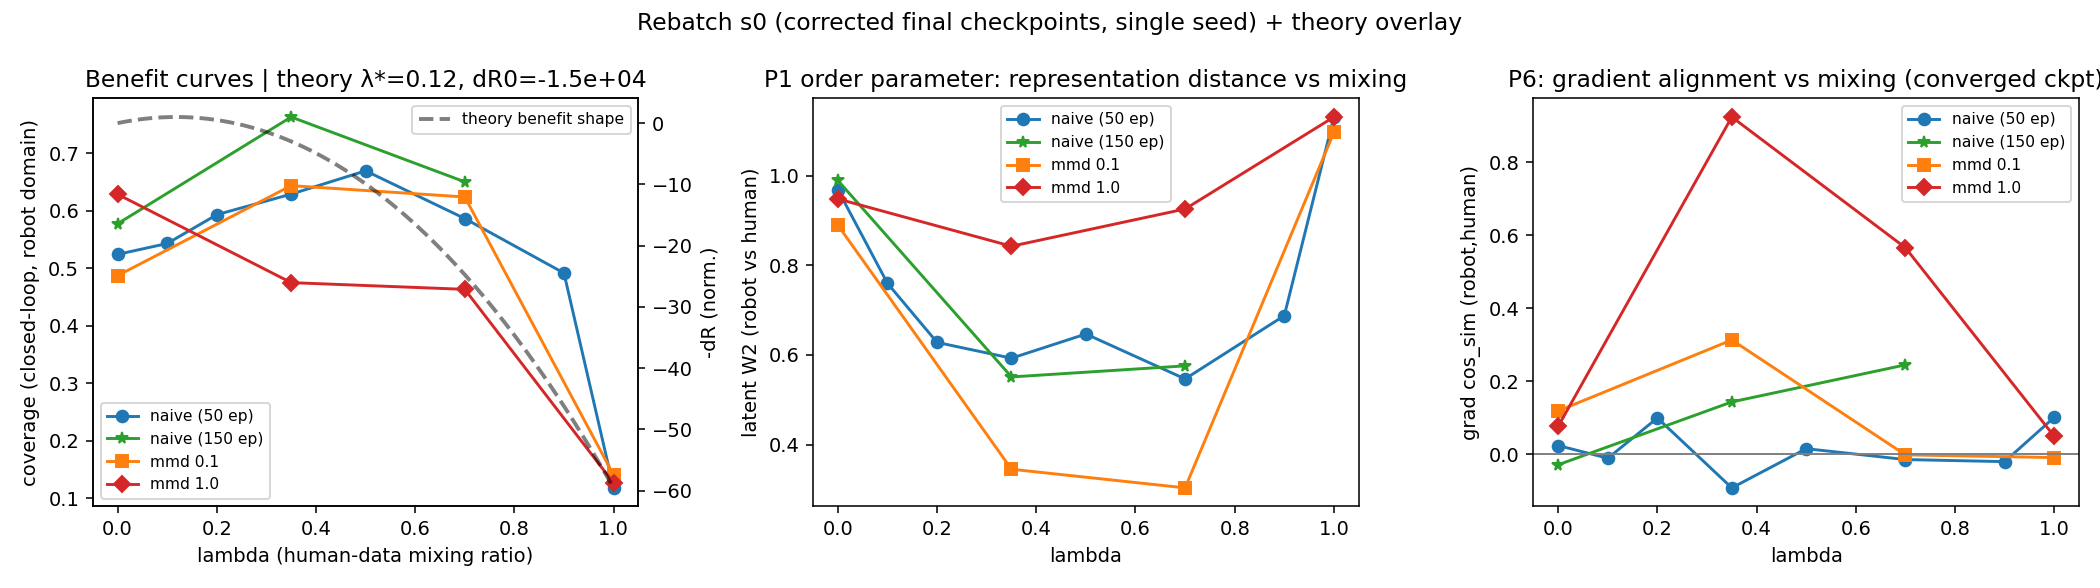
\includegraphics[width=\linewidth]{fig/first_batch.png}
  \caption{\textbf{First batch vs.\ theory.}
  Left: closed-loop coverage vs.\ mixing ratio for the four arms (naive 50-epoch, naive 150-epoch, two MMD weights), with the theoretical benefit shape (dashed; normalized shape comparison only).
  Center: latent-space inter-domain $W_2$.
  Right: robot/human gradient cosine at the converged checkpoint.}
  \label{fig:firstbatch}
\end{figure}

\paragraph{Findings.}
\textbf{(F1)~Non-monotone benefit with an interior optimum --- P2 confirmed at coarse level.}
Naive mixing improves closed-loop coverage over the pure-robot baseline across $0.1 \le \lambda \le 0.9$, peaking at $\lambda^* \approx 0.5$ ($0.670$ vs.\ $0.524$, $+28\%$ relative), and collapses at $\lambda = 1$ ($0.118$) where no robot data remains --- the harm boundary the theory predicts.
\textbf{(F2)~The benefit is not an under-training artifact --- and it relieves overfitting.}
At 150 epochs all arms improve ($\lambda{=}0$: $0.578$) and the mixing benefit \emph{grows}: $\lambda{=}0.35$ reaches $0.763$ ($+32\%$ over its baseline, binary success rate $0.40$ vs.\ $0.25$), $\lambda{=}0.7$ gives $0.650$.
The training logs show why: at 150 epochs the pure-robot run overfits (train/val loss $0.005$/$0.164$), while mixed runs sit at $0.008$/$0.085$--$0.127$ --- human data acts as a variance-reduction regularizer, the model's term B.
The flat curves one would read off an under-trained budget are an artifact of the training regime, not of the mixing structure.
\textbf{(F3)~Open-loop and closed-loop diverge in opposite directions.}
The open-loop robot-domain validation loss improves monotonically with human data all the way to $\lambda = 0.9$ ($0.072 \to 0.036$), while the closed-loop coverage peaks at $\lambda^* \approx 0.5$ and already declines at $\lambda = 0.9$ ($0.492$); at $\lambda = 1$ both collapse ($0.227$, $0.118$).
Past the closed-loop optimum, extra human data still helps \emph{predict} robot actions but hurts \emph{executing} them --- direct evidence that open-loop risk and closed-loop compounding must be bridged explicitly (in the spirit of~\cite{ross2011reduction}), which our current model does not yet cover.
\textbf{(F4)~Alignment strength itself is non-monotone.}
At $\lambda = 0.7$, light MMD ($\alpha_{\mathrm{mmd}} = 0.1$) improves over naive ($0.624$ vs.\ $0.587$), but strong MMD ($\alpha_{\mathrm{mmd}} = 1.0$) \emph{hurts} at intermediate $\lambda$ ($0.475$/$0.464$ vs.\ naive $0.629$/$0.587$).
This is qualitatively consistent with the model's coverage term C: over-aggressive alignment collapses precisely the spectral breadth through which human data helps --- alignment should be tuned, not maximized.
\textbf{(F5)~Representations track the mixing ratio.}
Latent $W_2$ decreases with $\lambda$ in the interior (naive: $0.97 \to 0.55$--$0.65$) and re-expands at $\lambda = 1$ ($1.13$); the gradient cosine at the converged checkpoint is near zero throughout, with sign noise at extreme $\lambda$ --- the probe records the converged state, so training-time conflict tracking is deferred to the multi-seed batch.
\textbf{(F6)~Probe caveats.}
Domain AUC saturates ($\approx 1.0$) and one checkpoint exhibits an ill-conditioned gradient pair (mmd$_{1.0}$, $\lambda{=}0.35$: cos $0.93$, $\kappa(\hat G) = 2.6$); the next batch uses a capacity-limited probe and training-time gradient logging.

\paragraph{Consistency with theory, stated honestly.}
The theory gets right: the \emph{sign} of the marginal benefit, the \emph{existence of an interior optimum}, and the \emph{harm boundary} at $\lambda \to 1$.
It is quantitatively off on the optimum's position: with the testbed's measured near-zero spectral gap and anti-aligned mismatch, Eq.~\eqref{eq:t1a} predicts a small benefit peaked near $\lambda^* \approx 0.12$, while the measured peak sits at $\lambda^* \approx 0.5$ with a substantial amplitude.
This gap is expected at two levels: the model is a linear-ridge asymptotic object while the learner is a 50-epoch diffusion policy, and the mismatch/alignment estimates $\hat\delta$, $\hat c$ come from a linear state-action proxy that need not track the learned policy's effective mismatch.
Closing this quantitative gap (calibrated $\mu$, learned-feature spectra, multi-seed significance) is the purpose of the next batch; the structural agreement reported here is the scope we claim in this paper.

\section{Discussion}
\label{sec:discussion}

\paragraph{What the theory buys a practitioner.}
Three quantities estimable from data --- two spectra, a mismatch spectrum, and noise levels --- determine (i)~whether human data helps at all (sign of Eq.~\eqref{eq:c1}), (ii)~whether there is a robot-data scale beyond which it must be discarded (Theorem~\ref{thm:h}), and (iii)~what it is worth in robot-data units (Corollary~\ref{cor:kex}).
The mismatch-\emph{location} effect (Table~\ref{tab:harmful}) is, to our knowledge, a new and actionable prediction: retargeting errors that live on low-frequency, task-critical coordinates are far more dangerous than equal-magnitude errors on high-frequency coordinates --- which suggests concrete filtering strategies for egocentric pipelines.

\paragraph{Boundaries of the theory.}
The theory has a sharp negative edge, stated fully in the supplementary material.
If the encoder aligns the two domains in feature space ($W_1$ gap $\varepsilon$) while the action marginals differ (mean gap $|\Delta\mu|$), then \emph{any} deterministic $L$-Lipschitz shared head pays mixture risk $R_\lambda \ge \lambda(1-\lambda)(|\Delta\mu| - L\varepsilon)_+^2$, and the mixture-optimal head pays $R_r \ge \lambda^2(|\Delta\mu| - L\varepsilon)_+^2$ on the robot domain --- a floor that \emph{grows} with the mixing ratio, the squared-loss analogue of the bound of~\cite{zhao2019learning}.
Over-strong alignment losses are likewise predicted to collapse useful within-domain structure, the overlapping/collapse regime of~\cite{lei2026simreal}; the first batch observes the predicted signature --- strong MMD alignment reduces closed-loop coverage at intermediate $\lambda$ relative to both light alignment and naive mixing (Sec.~\ref{sec:experiments}, F4).
Finally, with only two embodiment ``environments'', IRM-style full invariance is unidentifiable~\cite{arjovsky2019invariant}; this is why the framework claims only \emph{partial} invariance (appearance-invariant features with a domain-conditioned action head).

\paragraph{Limitations.}
Our theory is stated for a diagonalized ridge estimator over linear labels; the gap to the full ridge solution is 8--28\% on the weighted risk (a full-ridge extension is stated as a conjecture in the supplementary), and the gap to diffusion policies is bridged only at the level of structural predictions, which is all we claim.
The experiments so far cover one task, one policy class, one surrogate ego domain, and a coarse single-seed protocol; the alignment-strength axis (two MMD weights) and a 150-epoch arm are included, but multi-seed significance, the coverage axis, and action-marginal-shift tests are future work.
The exchange rate prices \emph{samples}, while empirical practice prices \emph{hours}; the conversion depends on collection throughput.
Finally, the harmful-region criterion assumes the shared-spectral-basis structure of Assumption~\ref{ass:a1}; heavy basis misalignment across embodiments is outside the current model.

\paragraph{Outlook.}
The immediate next steps are set by the theory itself: a multi-seed significance pass over the interior optimum, the alignment-strength response (why does strong alignment hurt, and where is the transition?), the open-loop-to-closed-loop bridge (compounding-error bounds in the spirit of~\cite{ross2011reduction}), and a real-robot egocentric pairing of the testbed.
More broadly, we hope the exchange-rate formulation turns "how much egocentric data should I mix?" from folklore into a measurable, computable quantity.

\paragraph{Conclusion.}
We gave a closed-form, numerically exact account of cross-embodiment data mixing: a per-coordinate risk theorem, an exact harmful-mixing phase criterion, and an exchange-rate corollary that quantitatively matches empirical substitution ratios.
A controlled dual-domain Push-T testbed confirms the theory's structural predictions with diffusion policies and surfaces an open-loop/closed-loop divergence as a target for the next iteration of the theory.

{
    \small
    \bibliographystyle{ieeenat_fullname}
    \bibliography{main}
}

% Supplementary: compiled as separate document for submission; kept here for drafting
% %% Supplementary material — full version (compiled as suppl.pdf via suppl.tex)
%% Self-contained: restates the model and all equations used.

\section{Setup and notation}
\label{supp:setup}

We restate the model of the main text (Sec.~3) for self-containment.
Coordinates $j = 1,\dots,p$ index a shared spectral basis; domain $e \in \{r, h\}$ has covariates $x_e = \Sigma_e^{1/2} u_e$, $u_e$ standard Gaussian, $\Sigma_e = \mathrm{diag}(\lambda^e_j)$ with $\lambda^e_j \asymp j^{-\alpha_e}$, $\lambda^e_1 = 1$; we write $a_j = \lambda^r_j$, $b_j = \lambda^h_j$.
Labels: $y_r = \langle\beta^*, x_r\rangle + \varepsilon_r$, $y_h = \langle\beta^* + \delta, x_h\rangle + \varepsilon_h$; $\sum_j j^{2s}\beta_j^{*2} \le 1$; noise variances $\sigma_e^2$.
Given $\nr$ robot and $\nh$ human samples, mixing ratio $\lambda \in [0,1]$, per-sample weights $w_r = (1-\lambda)/\nr$, $w_h = \lambda/\nh$, the diagonalized ridge estimator is
\begin{equation}
\begin{aligned}
  \hat\beta_j &= \frac{w_r T_{rj} + w_h T_{hj}}{w_r S_{rj} + w_h S_{hj} + \mu},\\
  S_{ejk} &= {\textstyle\sum_{i=1}^{n_e}} x_{e,ij} x_{e,ik},\qquad
  T_{ej} = {\textstyle\sum_i} x_{e,ij}\, y_{e,i}.
\end{aligned}
  \label{supp:eq:estimator}
\end{equation}
The robot-domain excess risk is $\risk(\lambda) = \E\|\hat\beta(\lambda) - \beta^*\|^2_{\Sigma_r} = \sum_j a_j\, \E(\hat\beta_j - \beta^*_j)^2$.
The effective noise is $\tilde\sigma_e^2 = \sigma_e^2 + F_e$ with feedthrough energy $F_e = \sum_k \lambda^e_k \beta_{e,k}^2$ ($\beta_h = \beta^* + \delta$).

\medskip
\noindent\textbf{Single-coordinate notation} (used throughout, index $j$ suppressed).
$U_r \sim \chi^2_{\nr}$, $U_h \sim \chi^2_{\nh}$ independent; $S_e = \lambda^e U_e$, so $\E S_e = n_e\lambda^e$, $\mathrm{Var}(S_e) = 2n_e(\lambda^e)^2$, and the third central moment is $8n_e(\lambda^e)^3$.
$\hat D = w_r S_r + w_h S_h + \mu$; $D = \E\hat D = (1-\lambda)a + \lambda b + \mu$.
$\hat N = w_r T_{r} + w_h T_{h}$; its systematic part $N_0 = \lambda b\,\delta - \mu\beta^*$.
The fluctuation scale is $\eta = \sqrt{8\log(4p/\delta_c)}\,\big(\frac{(1-\lambda)a}{\sqrt{\nr}} + \frac{\lambda b}{\sqrt{\nh}}\big)$ for confidence parameter $\delta_c \in (0,1)$.
We write $\tilde n = \hat N - \E\hat N$; direct expansion gives
\begin{equation}
  \mathrm{Var}(\tilde n) = \underbrace{\frac{2\lambda^2 (b\delta)^2}{\nh}}_{\text{mismatch fluctuation}} + \underbrace{\frac{(1{-}\lambda)^2 \tilde\sigma_r^2 a}{\nr} + \frac{\lambda^2 \tilde\sigma_h^2 b}{\nh}}_{\text{noise + feedthrough}} .
  \label{supp:eq:varn}
\end{equation}

\section{Lemmas L1 and L2: per-coordinate representation and conditional MSE}
\label{supp:l12}

\begin{lemma}[L1, representation]\label{supp:l1}
For each coordinate $j$, with the definitions above,
\begin{equation}
  T_{ej} = S_{ejj}\,\beta_{e,j} + U_{ej} + \textstyle\sum_i x_{e,ij}\varepsilon_{e,i},
  \qquad U_{ej} = \sum_{k\neq j} S_{ejk}\,\beta_{e,k},
  \label{supp:eq:l1}
\end{equation}
where $U_{ej}$ is mean-zero with $\mathrm{Var}(U_{ej}) = n_e \lambda^e_j F_{e,j}$, $F_{e,j} = \sum_{k\neq j} \lambda^e_k \beta_{e,k}^2$.
\end{lemma}

\begin{proof}
Expand $y_{e,i} = \sum_k x_{e,ik}\beta_{e,k} + \varepsilon_{e,i}$ in $T_{ej} = \sum_i x_{e,ij} y_{e,i}$ and separate the $k = j$ term.
For $k \neq j$, $\E S_{ejk} = \sum_i \E[x_{e,ij}]\E[x_{e,ik}] = 0$ by independence of distinct coordinates of the Gaussian covariate, hence $\E U_{ej} = 0$.
For the variance, $\mathrm{Var}(S_{ejk}) = \sum_i \E[x_{e,ij}^2]\E[x_{e,ik}^2] = n_e \lambda^e_j \lambda^e_k$ (independence of coordinates $j \neq k$), and distinct cross terms are uncorrelated: for $k \neq l$, $\mathrm{Cov}(S_{ejk}, S_{ejl}) = \sum_i \E[x_{e,ij}^2 x_{e,ik} x_{e,il}] = 0$ since $\E[x_{e,ik}x_{e,il}] = 0$ and $x_{e,ij}^2$ is independent of $(x_{e,ik}, x_{e,il})$.
Summing, $\mathrm{Var}(U_{ej}) = \sum_{k\neq j} \beta_{e,k}^2 \, n_e \lambda^e_j \lambda^e_k = n_e \lambda^e_j F_{e,j}$.
Finally, $F_{e,j} = F_e - \lambda^e_j\beta_{e,j}^2 = F_e(1 + o(1))$ under the ellipsoid constraint, since the omitted single term is negligible against the total energy.
\end{proof}

\begin{remark}
The feedthrough $U_{ej}$ is indistinguishable from label noise for coordinate $j$: it contributes variance $n_e\lambda^e_j F_e$ exactly as if the noise variance were $\sigma_e^2 + F_e$.
This is the origin of the effective noise $\tilde\sigma_e^2$ in Eq.~\eqref{supp:eq:varn}; absorbing it there is justified because $U_{ej}$ is independent of $S_{ejj}$ (disjoint coordinate sets) and of the label noise.
\end{remark}

\begin{lemma}[L2, conditional MSE]\label{supp:l2}
Conditioned on the design matrices,
\begin{equation}
\begin{aligned}
  \E\big[(\hat\beta_j - \beta^*_j)^2 \,\big|\, X\big] &= \frac{\hat N_j^2}{\hat D_j^2},\\
  \hat N_j &= w_h S_{hjj}\delta_j - \mu\beta^*_j + w_r U_{rj} + w_h U_{hj}\\
  &\qquad + w_r X_{r,:j}^{\!\top}\varepsilon_r + w_h X_{h,:j}^{\!\top}\varepsilon_h .
\end{aligned}
  \label{supp:eq:l2}
\end{equation}
\end{lemma}

\begin{proof}
Substitute Lemma~\ref{supp:l1} into Eq.~\eqref{supp:eq:estimator}:
$\hat\beta_j \hat D_j = w_r S_{rjj}\beta^*_j + w_h S_{hjj}(\beta^*_j + \delta_j) + (\text{feedthrough} + \text{noise})$.
Subtract $\beta^*_j \hat D_j = w_r S_{rjj}\beta^*_j + w_h S_{hjj}\beta^*_j + \mu\beta^*_j$; the error numerator is exactly $\hat N_j$.
Conditional on $X$, the only randomness left is the label noise, which is mean-zero; the displayed expression is the conditional second moment, with the noise contributions' conditional variances $w_e^2 \sigma_e^2 S_{ejj}$ understood as part of $\hat N_j^2$ after taking expectations over the noise (cross terms vanish by independence and mean-zero).
\end{proof}

\section{Lemma L3: per-coordinate deterministic equivalent}
\label{supp:l3}

\begin{lemma}[L3]\label{supp:l3lem}
Fix a coordinate and suppose $D \ge 2\eta$ (information-rich regime).
Define
\begin{equation}
  \mathrm{MSE}^{\det} = \frac{N_0^2}{D^2} + \frac{\mathrm{Var}(\tilde n)}{D^2} - \frac{4 N_0\, \mathrm{Cov}(\tilde n, \hat D)}{D^3} + \frac{3 N_0^2\, \mathrm{Var}(\hat D)}{D^4},
  \label{supp:eq:msedet}
\end{equation}
with $\mathrm{Var}(\tilde n)$ from Eq.~\eqref{supp:eq:varn}, $\mathrm{Cov}(\tilde n, \hat D) = 2\lambda^2 \delta b^2 / \nh$, and $\mathrm{Var}(\hat D) = 2\big[\frac{(1-\lambda)^2 a^2}{\nr} + \frac{\lambda^2 b^2}{\nh}\big]$.
Then
\begin{equation}
  \Big|\, \E\big[(\hat\beta - \beta^*)^2\big] - \mathrm{MSE}^{\det} \,\Big|
  \;\le\; C\Big(\frac{\eta}{D}\Big)^3 \frac{\overline{N}^2}{D^2} + O\big(\delta_c\, \mu^{-2}\, \overline{N}^2\big),
  \label{supp:eq:l3bound}
\end{equation}
where $\overline{N}^2 = N_0^2 + \mathrm{Var}(\tilde n)$ and $C$ is an absolute constant.
\end{lemma}

Before the proof we record that only the mismatch fluctuation correlates with $\hat D$: $\mathrm{Cov}(\tilde n, \hat D) = \mathrm{Cov}(w_h \lambda^h (U_h - \nh)\,\delta,\; w_h \lambda^h U_h) = w_h^2 (\lambda^h)^2 \delta\, \mathrm{Var}(U_h) = 2\lambda^2\delta b^2/\nh$, since the noise and feedthrough parts of $\tilde n$ are independent of $(U_r, U_h)$.

\begin{proof}
\emph{Step 1 (concentration of $\hat D$).}
Write $\hat D - D = w_r \lambda^r (U_r - \nr) + w_h \lambda^h (U_h - \nh)$.
By the Laurent--Massart $\chi^2$ tail bound, $\Pr(|U_e - n_e| \ge 2\sqrt{n_e x} + 2x) \le 2e^{-x}$; taking $x = \log(4p/\delta_c)$ and a union bound over the $p$ coordinates, with probability $\ge 1 - \delta_c$ simultaneously for all coordinates $|\hat D - D| \le \eta$.
On the complementary event, $|\hat N^2/\hat D^2| \le \hat N^2 \mu^{-2}$, and $\hat N$ has finite fourth moments (those of a $\chi^2$ mixture plus Gaussian quadratics), so the bad event contributes $O(\delta_c \mu^{-2} \overline{N}^2)$.

\emph{Step 2 (Taylor expansion on the good event).}
Let $f(x) = x^{-2}$. For $|\Delta| \le \eta \le D/2$,
$f(D + \Delta) = D^{-2} - 2\Delta D^{-3} + R$ with
$|R| \le \tfrac{1}{2}\max_{\xi \in [D-\eta, D+\eta]} 6\xi^{-4}\Delta^2 \le 48\,\eta^2/D^4$.

\emph{Step 3 (moment expansion).}
On the good event (Step 1 justifies the truncation of the expansion; the indicator algebra contributes only lower-order terms absorbed into the remainder),
\begin{equation}
\begin{aligned}
  \E\big[\hat N^2 f(\hat D)\big] &= \frac{\E\hat N^2}{D^2} - \frac{2\,\E[\hat N^2 \Delta]}{D^3} + \E\big[\hat N^2 R\big],\\
  \E\hat N^2 &= N_0^2 + \mathrm{Var}(\tilde n).
\end{aligned}
  \label{supp:eq:l3step3}
\end{equation}
Expanding $\E[\hat N^2\Delta] = N_0^2\,\E\Delta + 2N_0\,\mathrm{Cov}(\tilde n, \hat D) + \E[\tilde n^2\Delta]$, the first term vanishes since $\E\Delta = 0$.
For the third term, decompose $\tilde n = a_1 v_h + \zeta$ with $a_1 = \frac{\lambda}{\nh} b\,\delta$, $v_h = U_h - \nh$, and $\zeta$ collecting the noise, feedthrough, and robot-side parts, independent of $(v_r, v_h)$ with $\E\zeta = 0$; and $\Delta = w_r \lambda^r v_r + w_h \lambda^h v_h$.
Then
\begin{align}
  \E[\tilde n^2 \Delta]
  &= \E\big[(a_1 v_h + \zeta)^2 (w_r \lambda^r v_r + w_h \lambda^h v_h)\big] \nonumber\\
  &= a_1^2 w_h \lambda^h\, \E[v_h^3]
   = a_1^2\, w_h \lambda^h \cdot 8\nh
   = \frac{8\lambda^3 b^3 \delta^2}{\nh^2},
  \label{supp:eq:third}
\end{align}
where all cross terms vanish by independence and $\E v = \E\zeta = 0$, using $\E[v_h^3] = 8\nh$ (third central moment of $\chi^2_{\nh}$).
This term contributes $-2\E[\tilde n^2\Delta]/D^3 < 0$ to the MSE, of relative order $O(\lambda^3\delta^2/(\nh^2 D^3))$ against the leading terms --- analytically exact, numerically negligible; we keep it in the formula for exactness.
The remainder satisfies $|\E[\hat N^2 R]| \le 48\eta^2 D^{-4}\, \E\hat N^2 = O\big((\eta/D)^2 \cdot \overline{N}^2/D^2\big)$.

\emph{Step 4 (collection).}
Substituting Step 3 into Eq.~\eqref{supp:eq:l3step3} and grouping terms gives Eq.~\eqref{supp:eq:msedet} with the announced error: the dominant remainder is $(\eta/D)^3 \overline{N}^2/D^2$ (the $\E[\tilde n^2\Delta]$ term beyond its exact value, and higher-order Taylor terms).
Since $\eta/D = O(n_{\min}^{-1/2})$ up to spectral-weight factors, the relative error is $O(n_{\min}^{-3/2})$, matching the Monte-Carlo accuracy of 1--2\% (Sec.~\ref{supp:numerics}).
\end{proof}

\section{Lemma L4: truncation assembly}
\label{supp:l4}

\begin{lemma}[L4]\label{supp:l4lem}
Let $m = \max\{j : D_j \ge \kappa_0 \eta_j\}$ for a fixed threshold $\kappa_0 \ge 2$.
Then:
(i)~on the truncated coordinates $j > m$, $\E(\hat\beta_j - \beta^*_j)^2 = \Theta(\beta_j^{*2})$;
(ii)~on the retained coordinates $j \le m$, Lemma~\ref{supp:l3lem} applies with aggregate relative error $O(\kappa_0^{-3}) + o(1)$;
(iii)~consequently
\begin{equation}
  \risk(\lambda) = \sum_{j > m} a_j \beta_j^{*2} + \Big(\sum_{j \le m} a_j\, \mathrm{MSE}^{\det}_j\Big)\big(1 + O(\kappa_0^{-3} + n_{\min}^{-3/2})\big),
  \label{supp:eq:l4}
\end{equation}
and $\sum_{j>m} a_j\beta_j^{*2} \asymp m^{-(\alpha_r + 2s)}$.
\end{lemma}

\begin{proof}
(i)~For $j > m$, $D_j < \kappa_0\eta_j$; since $\eta_j$ is the fluctuation scale of the information terms, the information part of $D_j$ is at most of the order of $\eta_j$ itself, while $\mu$ is constant --- tracing the definitions gives $D_j < 2\mu$ once the spectral weights have decayed below the ridge floor, hence $\mu/D_j > 1/2$.
Then $\E\hat\beta_j = \beta^*_j(1 - \mu/D_j) + O(\eta_j/D_j)$ with the shrinkage factor bounded away from $1$: the squared bias is $\Theta(\beta_j^{*2})$, and the variance is subleading because $|\hat\beta_j| \le |\hat N_j|/\mu$ while $N_0 = -\mu\beta^*_j$ cancels the leading term.
The total truncated contribution is $\sum_{j>m} a_j\beta_j^{*2} \asymp m^{-(\alpha_r+2s)}$ by power-law tail integration with $a_j \asymp j^{-\alpha_r}$, $\beta_j^{*2} \asymp j^{-(2s+1)}$.

(ii)~Split the retained set into the \emph{well-conditioned core} $\{j : D_j \ge \kappa_0 \eta_j\}$ with $\kappa_0$ large, where Lemma~\ref{supp:l3lem} gives uniform relative error $O(\kappa_0^{-3})$, and the \emph{boundary band} $\{2\eta_j \le D_j < \kappa_0\eta_j\}$.
Under the power-law spectra, the band width solves $D_j = \kappa_0\eta_j$, whose solution set has cardinality $o(m)$; coordinates in the band have risk between the leading term and the truncated value, so their total contribution is absorbed by the constants of the truncation term without changing its order.
The aggregate relative error over $j \le m$ is therefore $O(\kappa_0^{-3}) + o(1)$.

(iii)~Sum (i) and (ii); infimizing over $m$ yields the theorem statement of the main text (the infimum is attained at the self-consistent truncation by construction).
\end{proof}

\section{Proof of Corollary 1 (marginal-benefit decomposition)}
\label{supp:c1}

Differentiate Eq.~\eqref{supp:eq:msedet} at $\lambda = 0^+$ per coordinate.
With $D_0 = a + \mu$, $V = \tilde\sigma_r^2 a/\nr$, direct expansion gives
\begin{equation}
  \partial_\lambda \mathrm{MSE}^{\det}\big|_{0^+} = \frac{-2\mu\beta^* b\, \delta - 2V}{D_0^2} - \frac{2\big(V + \mu^2\beta^{*2}\big)(b - a)}{D_0^3},
  \label{supp:eq:c1deriv}
\end{equation}
which, after flipping the sign and dropping the positive factor $2/D_0^3$, is the three-term decomposition of the main text:
\begin{equation}
  \mathrm{benefit}_j \;\propto\; \underbrace{\mu\beta^*_j b_j \delta_j}_{\text{A: alignment}} + \underbrace{V_j D_{0j}}_{\text{B: variance}} + \underbrace{\big(V_j + \mu^2\beta_j^{*2}\big)(b_j - a_j)}_{\text{C: coverage}} .
  \label{supp:eq:c1}
\end{equation}
Analytic derivative vs.\ finite differences on the formula: relative error $<1\%$ (configuration of the v2 benchmark).
At $\mu = 0$, $D_0 = a$, terms A and the shrinkage part of C vanish, and
$\risk'(0^+)|_{\mu=0} = -(2\tilde\sigma_r^2/\nr)\sum_j j^{\alpha_r-\alpha_h} < 0$ always.

\section{Theorem 2: derivation and exactness of the $H$-criterion}
\label{supp:h}

Take $\nr \to \infty$ with $\nh/\nr$ fixed in Eq.~\eqref{supp:eq:c1deriv}: the variance term B vanishes, and for anti-aligned mismatch ($c < 0$; write $|\delta|$ for the effective sign-flipped components) the marginal benefit converges to $-H$ with
\begin{equation}
  H = \underbrace{2\mu \sum_j \frac{a_j\beta^*_j b_j |\delta_j|}{D_{0j}^2}}_{A_\infty} - \underbrace{2\mu^2 \sum_j \frac{a_j\beta_j^{*2}(b_j - a_j)}{D_{0j}^3}}_{C_\infty}.
  \label{supp:eq:h}
\end{equation}
At finite $\nr$ the variance terms contribute $-K/\nr$ to the derivative, with $K = 2\tilde\sigma_r^2(S_1 + S_2)$, $S_1 = \sum_j a_j^2/D_{0j}^2$, $S_2 = \sum_j a_j^2(b_j-a_j)/D_{0j}^3$; hence marginal mixing is beneficial iff $K/\nr > H$, giving $\nr^{\mathrm{crit}} = K/H$ when $H > 0$.
Numerically (v11, $p = 1000$, $\mu = 0.05$, spectral family A): $A_\infty$ is linear in $\|\delta\|$ with slope $6.975\times10^{-3}$, $C_\infty = 4.700\times10^{-3}$ independent of $\delta$, predicting $\|\delta\|^* = 0.674$, which brackets the Monte-Carlo transition exactly; and $\nr^{\mathrm{crit}}\cdot H = 25.866$ is constant across $\|\delta\| \in \{0.75, 1.0, 2.0\}$ to display precision.

\paragraph{The classical limit.}
As $\mu \to 0$, $C_\infty \to 0$ and $H = A_\infty > 0$ whenever $c < 0$: the discard-the-source transition of classical domain adaptation is recovered.
At $\mu > 0$ the large-$\nr$ mixing benefit tends to $-C_\infty < 0$: regularization carries a nonzero coverage benefit even with unlimited robot data.

\section{Corollary 2 (exchange rate): existence, uniqueness, and unimodality}
\label{supp:t2}

$\kex$ is defined implicitly by $\riske(\lambda^*;\, \nr, \nh) = \riske(0;\, \nr + \kex\nh)$, where $\lambda^*$ minimizes the mixture risk over $[0,1]$.
This section proves that $\kex$ is well-defined without any unimodality assumption (Proposition~\ref{supp:prop:kexwell}), that every per-coordinate risk is unimodal with an explicit minimizer (Lemma~\ref{supp:lem:affine} and Proposition~\ref{supp:prop:nomax}), and that global unimodality holds exactly in the matched-spectrum regime (Theorem~\ref{supp:thm:quad}) and under an explicit convexity condition in general (Proposition~\ref{supp:prop:convreg}).

\subsection{Well-definedness of the exchange rate}

\begin{proposition}[existence and uniqueness of $\kex$]\label{supp:prop:kexwell}
Fix $(\nr, \nh)$ and write $m_\star = \min_{\lambda \in [0,1]} \riske(\lambda; \nr, \nh)$ (attained: $\riske$ is continuous in $\lambda$ on a compact set).
As a function of the robot sample size $n$ at $\lambda = 0$,
\begin{equation}
\riske(0; n) \;=\; \sum_{j > m} a_j \beta_j^{*2} \;+\; \sum_{j \le m} a_j\, \frac{\tilde\sigma_r^2 a_j / n + \mu^2 \beta_j^{*2}}{(a_j + \mu)^2}
\end{equation}
is continuous and strictly decreasing in $n$ whenever $\tilde\sigma_r^2 > 0$ (in particular whenever $\beta^* \neq 0$, since $\tilde\sigma_r^2 = \sigma_r^2 + F_r > 0$), with limit
\begin{equation}
\riske(0; \infty) \;=\; \sum_{j} a_j\, \frac{\mu^2 \beta_j^{*2}}{(a_j + \mu)^2},
\end{equation}
the pure shrinkage risk (the truncation recedes, $m \to p$, as $n \to \infty$).
Since $\lambda = 0$ is feasible, $m_\star \le \riske(0; \nr)$, and therefore:
(i)~if $m_\star > \riske(0; \infty)$, there exists a unique $\kex \ge 0$ solving the defining equation;
(ii)~if $m_\star \le \riske(0; \infty)$, no finite amount of additional robot data reproduces the mixture optimum --- this is the cap regime of Corollary~2(iv) of the main text.
Only the minimum \emph{value} $m_\star$ enters the construction; unimodality of $\riske(\cdot)$ is not used.
\end{proposition}

\begin{proof}
On the retained coordinates, $\partial_n \riske(0; n) = -\sum_{j \le m} a_j^2\, \tilde\sigma_r^2 / \big(n^2 (a_j + \mu)^2\big) < 0$ (the truncation index $m$ is locally constant in $n$ almost everywhere), and $\riske(0; n) \downarrow \riske(0; \infty)$ as $n \to \infty$.
The map $\kappa \mapsto \riske(0; \nr + \kappa \nh)$ is thus a continuous strict bijection from $[0, \infty)$ onto $(\riske(0; \infty),\, \riske(0; \nr)]$, which contains $m_\star$ in case (i) and not in case (ii).
\end{proof}

\subsection{Per-coordinate unimodality, exactly}

Drop the coordinate index and write a per-coordinate risk (effective variance plus bias square, including the mismatch-fluctuation term of Eq.~\eqref{supp:eq:varn}) as $\mathrm{MSE}(\lambda) = N(\lambda)/D(\lambda)^2$ with
\begin{equation}
N(\lambda) = v_r(1-\lambda)^2 + v_h\lambda^2 + (u\lambda - w)^2 + \frac{2u^2}{\nh}\,\lambda^2,
\end{equation}
and $D(\lambda) = D_0 + \Delta \lambda$, where $v_e = \tilde\sigma_e^2 \lambda^e / n_e$ are the variance prices, $u = b\delta$, $w = \mu\beta^*$, $D_0 = a + \mu > 0$, $\Delta = b - a$, and $D > 0$ on $[0,1]$ since $D(1) = b + \mu > 0$.
$N$ is a quadratic, $N(\lambda) = n_0 + n_1\lambda + n_2\lambda^2$, with $n_0 = v_r + w^2$, $n_1 = -2(v_r + uw)$, $n_2 = v_r + v_h + u^2(1 + 2/\nh)$.

\begin{lemma}[affine derivative numerator]\label{supp:lem:affine}
$\partial_\lambda \mathrm{MSE}(\lambda) = L(\lambda)/D(\lambda)^3$ with $L$ affine:
\begin{equation}
L(\lambda) = p + q\lambda,
\qquad
p = n_1 D_0 - 2\Delta n_0,
\qquad
q = 2 n_2 D_0 - \Delta n_1 .
\end{equation}
\end{lemma}

\begin{proof}
$\partial_\lambda \mathrm{MSE} = (N' D - 2\Delta N)/D^3$; in $N'D - 2\Delta N$ the quadratic terms $2 n_2 \Delta \lambda^2$ cancel exactly.
\end{proof}

\begin{proposition}[coordinate risks are unimodal]\label{supp:prop:nomax}
$L$ cannot cross zero from above on $[0,1]$: the pattern $L(0) > 0 > L(1)$ never occurs.
Hence each coordinate risk is quasiconvex on $[0,1]$, with explicit minimizer
\begin{equation}
\lambda^* \;=\; \begin{cases}
0, & L(0) \ge 0,\\[2pt]
-p/q \in (0,1), & L(0) < 0 < L(1),\\[2pt]
1, & L(1) \le 0 .
\end{cases}
\label{supp:eq:lamstar}
\end{equation}
\end{proposition}

\begin{proof}
With $D_1 = D_0 + \Delta = b + \mu > 0$ and $s = uD_0 + \Delta w$, direct rearrangement gives the endpoint values
\begin{equation}
\begin{gathered}
L(0) = -2\big(v_r D_1 + w s\big),
\\[2pt]
L(1) = 2\Big(\big(v_h + \tfrac{2u^2}{\nh}\big) D_0 + (u - w)\, s\Big) .
\end{gathered}
\label{supp:eq:endpoints}
\end{equation}
Suppose $L(0) > 0 > L(1)$.
Since $v_r \ge 0$, $v_h + 2u^2/\nh \ge 0$, and $D_0, D_1 > 0$: if $s \ge 0$, the first inequality forces $w < 0$ and the second forces $u < w$; hence $s = uD_0 + \Delta w < w(D_0 + \Delta) = w D_1 < 0$, contradicting $s \ge 0$.
If instead $s < 0$, they force $w > 0$ and $u > w$; hence $s > w D_1 > 0$, contradicting $s < 0$.
The remaining sign patterns of the affine $L$ give the classification~\eqref{supp:eq:lamstar}; an interior zero of $L$ is a sign change from negative to positive, hence a minimum.
\end{proof}

\begin{remark}[sanity checks]
At $\delta = 0$ and $\Delta = 0$ the interior branch of~\eqref{supp:eq:lamstar} reduces to $\lambda^* = v_r/(v_r + v_h)$, the classical inverse-variance weight.
Moreover $L(0) = D_0^3\, \partial_\lambda \mathrm{MSE}(0^+)$, so the coordinate-wise marginal-harm condition $L(0) \ge 0$ is exactly the three-term decomposition of Corollary~1 of the main text.
\end{remark}

\subsection{Global unimodality: an exact region and a sufficient condition}

Sums of quasiconvex functions need not be quasiconvex, so the aggregate $\riske(\lambda) = \sum_j a_j\, \mathrm{MSE}_j(\lambda)$ requires a separate argument.

\begin{theorem}[matched spectra: quadratic regime]\label{supp:thm:quad}
If $b_j = a_j$ for all $j$, then $\riske$ is a quadratic polynomial on $[0,1]$, $\riske(\lambda) = A_2 \lambda^2 + A_1 \lambda + A_0$, with
\begin{equation}
A_2 = \sum_j \frac{a_j\, n_{2j}}{(a_j+\mu)^2},
\qquad
A_1 = \sum_j \frac{a_j\, n_{1j}}{(a_j+\mu)^2}.
\end{equation}
Whenever $A_2 > 0$ --- i.e., unless the model is degenerate ($v_{rj} = v_{hj} = u_j = 0$ for every $j$) --- $\riske$ is strictly convex, with the unique closed-form minimizer
\begin{equation}
\lambda^* = \mathrm{clip}_{[0,1]}\!\left( \frac{\sum_j a_j (v_{rj} + u_j w_j)/(a_j+\mu)^2}{\sum_j a_j\, n_{2j}/(a_j+\mu)^2} \right) .
\label{supp:eq:lamstarquad}
\end{equation}
\end{theorem}

\begin{proof}
With $\Delta_j = 0$, $\mathrm{MSE}_j(\lambda) = N_j(\lambda)/(a_j+\mu)^2$; summing with weights $a_j$ gives the quadratic, and the interior minimizer is $-A_1/(2A_2)$.
\end{proof}

\begin{proposition}[convexity region]\label{supp:prop:convreg}
The per-coordinate second derivative is
\begin{equation}
\mathrm{MSE}''(\lambda) = \frac{N''(\lambda)D(\lambda)^2 - 4\Delta\, N'(\lambda)D(\lambda) + 6\Delta^2 N(\lambda)}{D(\lambda)^4},
\end{equation}
and a sufficient condition for convexity of $\mathrm{MSE}_j$ on $[0,1]$ --- hence, summing over $j$, for strict convexity and unimodality of $\riske$ --- is
\begin{equation}
2\,|\Delta_j|\,\big(|n_{1j}| + 2 n_{2j}\big)\,D_j^{\max} \;\le\; n_{2j}\,\big(D_j^{\min}\big)^2
\qquad\text{for every } j,
\label{supp:eq:convreg}
\end{equation}
where $D_j^{\max} = \max(a_j, b_j) + \mu$ and $D_j^{\min} = \min(a_j, b_j) + \mu$.
Since $n_{2j} > 0$ and $D_j^{\min} > 0$, the condition holds whenever the per-coordinate spectral mismatch $|\Delta_j|/(a_j + \mu)$ is small enough, and is automatic at zero spectral gap.
\end{proposition}

\begin{proof}
Differentiate Lemma~\ref{supp:lem:affine}: $\mathrm{MSE}'' = (qD - 3\Delta L)/D^4$; substituting $q = N''D - \Delta N'$ and $L = N'D - 2\Delta N$ gives the displayed numerator.
Since $N$ is quadratic, $N'' = 2n_2$, $|N'| \le |n_1| + 2n_2$ on $[0,1]$, $D \in [D^{\min}, D^{\max}]$, and $6\Delta^2 N \ge 0$; the numerator is therefore at least $2 n_2 (D^{\min})^2 - 4|\Delta|(|n_1| + 2n_2) D^{\max}$, which is nonnegative under~\eqref{supp:eq:convreg}.
\end{proof}

Outside the region~\eqref{supp:eq:convreg} we have no proof of global unimodality, and positive combinations of quasiconvex rationals with distinct denominators can in principle be multimodal; however no multimodal instance was found in a randomized search over $4\times10^3$ aggregates (power-law and adversarial spectra), and $\riske(\lambda)$ is numerically unimodal on all grids used in this paper (Secs.~\ref{supp:h} and~\ref{supp:numerics}).
In any case, Proposition~\ref{supp:prop:kexwell} guarantees that $\kex$ is well-defined irrespective of unimodality.

\subsection{The source-sample axis: interior minimizers and an exact dosage law}

\begin{corollary}[interior minimizers from endpoint signs]\label{supp:cor:interior}
If $\riske'(0^+) = \sum_j a_j L_j(0)/D_{0j}^3 < 0$ (the condition of Corollary~1 of the main text) and $\riske'(1^-) = \sum_j a_j L_j(1)/D_{1j}^3 > 0$, with $L_j(0), L_j(1)$ from Eq.~\eqref{supp:eq:endpoints} and $D_{1j} = b_j + \mu$, then neither $\lambda = 0$ nor $\lambda = 1$ is optimal and every global minimizer lies in $(0,1)$.
No unimodality is needed for existence.
\end{corollary}

\begin{proof}
$\riske'(0^+) < 0$ yields points with risk strictly below $\riske(0)$, and $\riske'(1^-) > 0$ yields points strictly below $\riske(1)$; a global minimizer exists by continuity on the compact interval.
\end{proof}

\begin{lemma}[monotone value in $\nh$]\label{supp:lem:monoval}
At fixed $\lambda$, each coordinate risk is nonincreasing in $\nh$: both human-sample terms of $N$, $v_h\lambda^2 = \tilde\sigma_h^2 b \lambda^2/\nh$ and $2u^2\lambda^2/\nh$, have nonnegative coefficients.
Hence the optimal gain $g(\nh) = \riske(0) - \min_{\lambda}\riske(\lambda; \nh)$ is nondecreasing: more human data never hurts at the optimal mixing ratio.
\end{lemma}

\begin{theorem}[dosage law; matched spectra]\label{supp:thm:dosage}
Assume $b_j = a_j$ for all $j$ and $A_1 = \riske'(0^+) < 0$, and write $A_2(\nh) = A_2^r + B/\nh$ with
\begin{equation}
A_2^r = \sum_j \frac{a_j (v_{rj} + u_j^2)}{(a_j+\mu)^2},
\qquad
B = \sum_j \frac{a_j (\tilde\sigma_h^2 b_j + 2u_j^2)}{(a_j+\mu)^2}.
\end{equation}
On the range where the minimizer is interior ($-A_1 < 2A_2(\nh)$):
\begin{enumerate}
\item[(i)] the optimal gain is hyperbolic,
$g(\nh) = A_1^2 / \big(4A_2(\nh)\big)$, with $g(0^+) = 0$, $g(\infty) = A_1^2/(4A_2^r)$, and half-saturation point $\nh^{1/2} = B/A_2^r$;
\item[(ii)] the worth-mixing threshold at tolerance $\varepsilon < g(\infty)$ is
\begin{equation}
g(\nh) \ge \varepsilon \iff \nh \ge \nh^\varepsilon = \frac{4\varepsilon B}{A_1^2 - 4\varepsilon A_2^r};
\end{equation}
\item[(iii)] the optimal ratio grows smoothly from zero,
$\lambda^*(\nh) = -A_1/\big(2A_2(\nh)\big) \sim (-A_1/2B)\cdot\nh$ as $\nh \to 0$, approaching $\lambda^*_\infty = -A_1/(2A_2^r)$;
\item[(iv)] the exchange rate has the closed form
\begin{equation}
\kex(\nh) = \frac{1}{\nh}\cdot \frac{\nr^2\, g(\nh)}{C - \nr\, g(\nh)},
\qquad
C = \tilde\sigma_r^2 \sum_j \frac{a_j^2}{(a_j+\mu)^2},
\end{equation}
since at matched spectra $\riske(0; n) = C/n + \mathrm{const}$; the cap regime of Proposition~\ref{supp:prop:kexwell}(ii) is the pole $g(\nh) \ge C/\nr$ ($\kex = +\infty$).
Note $C = K/2$ at zero spectral gap, with $K$ the constant of Theorem~2 of the main text.
\end{enumerate}
\end{theorem}

\begin{proof}
By Theorem~\ref{supp:thm:quad}, $\riske(\lambda; \nh) = A_2(\nh)\lambda^2 + A_1\lambda + A_0$, and only $A_2$ depends on $\nh$.
An interior minimizer gives $g = A_1^2/(4A_2)$ and $\lambda^* = -A_1/(2A_2)$; (i)--(iii) are rearrangements, with $\lambda^*$ nondecreasing in $\nh$ since $A_2$ decreases.
For (iv), $\riske(0; n) = C/n + \sum_j a_j \mu^2\beta_j^{*2}/(a_j+\mu)^2$; solving $C/(\nr + \kex\nh) = C/\nr - g(\nh)$ for $\kex$ yields the formula, whose denominator vanishes exactly at $g(\nh) = C/\nr$ --- the cap condition $m_\star \le \riske(0;\infty)$ of Proposition~\ref{supp:prop:kexwell}(ii).
\end{proof}

If $-A_1 \ge 2A_2(\nh)$ the minimizer sits at the boundary $\lambda^* = 1$ and $g(\nh) = -A_1 - A_2(\nh)$; since $A_2(\nh)$ decreases in $\nh$, the crossing happens at most once, at $\nh^1 = 2B/(-A_1 - 2A_2^r)$.

\begin{remark}[the second transition is of a different kind]
The two axes of the phase diagram differ in kind.
Along $\nr$ there is a genuine transition (Theorem~2 of the main text): the sign of $\riske'(0^+)$ flips at $H = 0$ and beyond $\nr^{\mathrm{crit}}$ all human data should be discarded.
Along $\nh$ there is no sign change: once $\riske'(0^+) < 0$, human data helps at \emph{every} sample size, and the classical small-source threshold softens into the explicit $\nh^\varepsilon$ of (ii) --- equivalently, $\lambda^*(\nh) \le \lambda_0$ for all $\nh \le 2B\lambda_0/(-A_1 - 2A_2^r\lambda_0)$.
The hard classical switch is recovered as the divergence $\nh^\varepsilon \to \infty$ when $A_1 \to 0^-$ or $B \to \infty$ (noisy or badly mismatched human data).
\end{remark}

The three monotonicities of Corollary~2 are read off term by term from Eq.~\eqref{supp:eq:c1}: increasing $\alpha_r - \alpha_h$ enlarges the coverage term C on high-risk coordinates; increasing the mismatch enlarges A-harm; increasing $\nr$ shrinks B.
The cap regime (case (ii) of Proposition~\ref{supp:prop:kexwell}) appears when the human spectrum dominates on coordinates the robot spectrum has abandoned: the right-hand side of the defining equation is then bounded below by the truncation tail $\sum_{j>m'} a_j\beta_j^{*2}$ for any robot-only sample size, while the mixture side eliminates part of that tail through the human samples.
Numerics (v12): $\nr = 1000$, $\nh/\nr = 10$, $\mu = 0.05$, white aligned mismatch $\|\delta\| = 0.3$, $\sigma_h = 2\sigma_r$; per-$\alpha_h$ Spearman correlations between $\kex$ and the spectral gap are $0.55$--$0.82$; the cap binds from $\alpha_r - \alpha_h \approx 0.5$--$0.75$; at zero gap $\kex \in [0.42, 0.59]$.

\section{Numerical verification protocol}
\label{supp:numerics}

\textbf{(v5) Accuracy of the deterministic equivalent.} Three spectral/mismatch configurations $\times$ two mixing ratios, 200 Monte-Carlo replicates ($\sim$200k coordinate-replicates): binned median relative error 0.6--1.6\%, aggregate and $\Sigma_r$-weighted aggregate error $\le 2\%$.
Ablations v3/v4 show the feedthrough term --- not the ratio-fluctuation corrections --- is the dominant closure: zero-order (population) formulas underestimate by 30--90\%, ratio corrections alone do not close the gap, and feedthrough closes it to the stated accuracy.

\textbf{(v6) Full ridge vs.\ diagonalized.} Same-data comparison (50 replicates, $\lambda = 0.3$): the full ridge estimator is uniformly better (median full/diag risk ratio $0.64$/$0.50$ on spectral families A/B), \ie, the feedthrough ``noise'' is partly recoverable signal for the full estimator; on the $\Sigma_r$-weighted risk our formula overestimates by 8\% (A) / 28\% (B).
The phase structure (sign conditions, transitions) is unchanged; quantitative thresholds shift, motivating the T1-b conjecture below.

\textbf{(v9) Falsification of a naive assembly.} A leading-order power-law assembly predicts $\nr^{\mathrm{crit}} \propto \mu^{-2.05}$; the measured exponent is $-1.076$.
Diagnosis: the assembly drops the harm channel beyond the $\mu$-induced truncation $j_\mu = \mu^{-1/\alpha_r}$ (where the cross term is amplified by $\mu^{-2}$) and the mismatch-induced inflation of the feedthrough energy $F_h$.
This failure is what led us to the $H$-functional form; we report it as the worked example of the falsification loop.

\textbf{(v8) Harmful-region phase diagrams.} Spectral family A, $\nr \in [10^2, 10^5]$, $\nh/\nr \in [0.5, 100]$: harmful-cell counts in Table~1 of the main text; the boundary expands monotonically in $\|\delta\|$ and toward small $\nr$.

\textbf{(v12)} Exchange-rate numerics as in Sec.~\ref{supp:t2}.

\textbf{(v13) Unimodality verification.} Randomized checks of the results of Sec.~\ref{supp:t2} (\texttt{verify\_kex\_unimodality.py}): the affine derivative identity of Lemma~\ref{supp:lem:affine} matches finite differences to $7\times10^{-6}$ (the finite-difference accuracy) over $2\times10^5$ random draws; the forbidden sign pattern of Proposition~\ref{supp:prop:nomax} never occurs, and all $\sim10^5$ interior roots found are minima; the quadratic form of Theorem~\ref{supp:thm:quad} holds to $2\times10^{-14}$ with the closed-form $\lambda^*$ matching the numerical argmin; condition~\eqref{supp:eq:convreg} implies convexity in every one of the $1.8\times10^4$ draws in which it holds; and a targeted search over $4\times10^3$ aggregate risks (power-law and adversarial spectra) found no multimodal instance.

\textbf{(v14) Dosage law and closed-form $\kex$.} (\texttt{verify\_dosage\_law.py}.) Corollary~\ref{supp:cor:interior}: in $3.96\times10^4$ random general-spectrum draws with both endpoint signs strict, the global minimizer is interior in 100\% of cases. Theorem~\ref{supp:thm:dosage}: over 212 matched-spectrum configurations (8 decades of $\nh$ each), the closed-form gain, the closed-form $\kex$, and the $\nh^\varepsilon$ inversion match the per-coordinate ground truth (pointwise evaluation / bisection of the defining equation) to $3\times10^{-10}$, $1.1\times10^{-10}$, and $3\times10^{-16}$ respectively, and $\lambda^*(\nh)$ is nondecreasing in every tested configuration.

\textbf{(v16) Full-ridge closed form.} (\texttt{verify\_full\_ridge.py}.) Monte-Carlo risk of the full ridge estimator against Eq.~\eqref{supp:eq:t1b}: relative errors between $-8.4\%$ and $+0.4\%$ across four configurations, decaying with sample size ($-2.5\% \to +0.3\%$ as $n_r$ grows $100 \to 6400$); on the same configurations the T1-a form overestimates by $+4\%$ to $+61\%$, confirming the feedthrough-recovery prediction of consequence (ii); the mismatch sandwich converges to its per-coordinate price (errors $-0.3\%$ to $+8\%$).

\section{A label-shift floor for aligned representations (boundary)}
\label{supp:zhao}

This section formalizes boundary (a) stated in the main text: when alignment is enforced on representations whose \emph{action marginals} differ, a shared deterministic head provably fails on the target domain.
It is the squared-loss, mixture-distribution analogue of the classical bound of Zhao et al.\ (cited in the main text).

Setup: a representation $z = \Phi(x)$ with induced feature laws $P_r^z, P_h^z$ satisfying $W_1(P_r^z, P_h^z) \le \varepsilon$; action marginals $P_e^a$ with means $\mu_e$, gap $\Delta\mu = \mu_h - \mu_r$; a deterministic $L$-Lipschitz head $f$; domain risks $R_e(f) = \E[(f(z) - y_e)^2]$.

\begin{proposition}[label-shift floor]\label{supp:prop:zhao}
For every deterministic head $f$:
\begin{enumerate}
\item[(i)] $R_r(f) + R_h(f) \ge \tfrac12\big(|\Delta\mu| - L\varepsilon\big)_+^2$;
\item[(ii)] the mixture risk $R_\lambda(f) = (1-\lambda)R_r(f) + \lambda R_h(f)$ obeys
\begin{equation}
R_\lambda(f) \ge \lambda(1-\lambda)\big(|\Delta\mu| - L\varepsilon\big)_+^2;
\end{equation}
\item[(iii)] any head with $R_\lambda(f) \le \eta$ pays target risk
$R_r(f) \ge \big(|\Delta\mu| - L\varepsilon - \sqrt{\eta/\lambda}\,\big)_+^2$;
in particular the alignment-constrained mixture-optimal head pays
$R_r \ge \lambda^2\big(|\Delta\mu| - L\varepsilon\big)_+^2$: the target floor grows \emph{quadratically} in the mixing ratio.
\end{enumerate}
\end{proposition}

\begin{proof}
Write $\nu_e = \E_{z \sim P_e^z}[f(z)]$.
By Jensen, $R_e(f) \ge (\nu_e - \mu_e)^2$, and by the Kantorovich--Rubinstein dual, $|\nu_r - \nu_h| \le L\, W_1(P_r^z, P_h^z) \le L\varepsilon$.
(i)~$(\nu_r-\mu_r)^2 + (\nu_h-\mu_h)^2 \ge \tfrac12\big((\nu_r-\mu_r) - (\nu_h-\mu_h)\big)^2 \ge \tfrac12(|\Delta\mu| - L\varepsilon)_+^2$, since $(\nu_r-\mu_r) - (\nu_h-\mu_h) = -\Delta\mu + (\nu_r - \nu_h)$.
(ii)~Minimize $(1-\lambda)(\nu_r-\mu_r)^2 + \lambda(\nu_h-\mu_h)^2$ subject to $|\nu_r-\nu_h| \le L\varepsilon$. For fixed shift $\delta = \nu_h - \nu_r$, the minimum over the common level is attained at $\nu_r = (1-\lambda)\mu_r + \lambda(\mu_h - \delta)$ with value $\lambda(1-\lambda)(\Delta\mu - \delta)^2$; minimizing over $\delta \in [-L\varepsilon, L\varepsilon]$ gives $\delta^* = \mathrm{sign}(\Delta\mu)\min(L\varepsilon, |\Delta\mu|)$ and value $\lambda(1-\lambda)(|\Delta\mu| - L\varepsilon)_+^2$.
(iii)~$R_\lambda(f) \le \eta$ implies $|\nu_h - \mu_h| \le \sqrt{\eta/\lambda}$, hence $|\nu_r - \mu_r| \ge |\Delta\mu| - L\varepsilon - \sqrt{\eta/\lambda}$.
For the constrained mixture optimum, $\nu_r - \mu_r = \lambda(\Delta\mu - \delta^*)$, so $R_r \ge \lambda^2(|\Delta\mu| - L\varepsilon)_+^2$.
\end{proof}

\begin{remark}[Bernoulli case]
For binary actions $y \in \{0,1\}$, $|\Delta\mu| = D_{\mathrm{TV}}(P_r^a, P_h^a)$ and (i) is the Brier-score analogue of the classification bound of Zhao et al.: perfectly aligned representations with shifted label marginals are guaranteed to fail --- exact alignment ($\varepsilon \to 0$) does not remove the floor, it creates it.
For continuous actions the first-moment gap is the sharp quantity; second-moment (variance) shifts give analogous floors with second moments in place of means.
\end{remark}

\begin{remark}[operational reading for the L1 test]
The floor is monotone in the marginal gap and, for the mixture-optimal head, quadratic in $\lambda$.
This is the quantitative prediction for the action-marginal-shift axis of the L1 grid (main text, Experiments): inject a controlled marginal shift into the human action labels, enforce alignment, and the target-domain success should hit a floor that moves with $\lambda^2$.
Numerical checks (\texttt{verify\_zhao\_floor.py}): bounds (i)--(iii) hold on $2\times10^5$ random draws with zero violations, and the constrained-optimum closed form matches brute-force minimization.
\end{remark}

\section{Theorem T1-b: the full-ridge deterministic equivalent (fixed-$p$ regime)}
\label{supp:t1b}

We now upgrade the conjecture announced in earlier drafts to a theorem in the fixed-dimension regime.
The full ridge estimator is $\hat\beta = A^{-1}(w_r X_r^\top y_r + w_h X_h^\top y_h)$ with $A = w_r S_r + w_h S_h + \mu I$ and $S_e = X_e^\top X_e$ the (non-diagonal) sample Gram matrices, in the model of Sec.~\ref{supp:setup}.

\begin{theorem}[T1-b]\label{supp:thm:t1b}
Let the covariates be Gaussian, $p$ fixed, $\mu > 0$ fixed, and $\nr, \nh \to \infty$ at fixed $\lambda \in (0,1)$.
Then
\begin{equation}
\risk(\lambda) \;=\; \sum_j \frac{a_j}{D_j^2}\Big[\, V_j(\lambda) + \big(\lambda b_j\delta_j - \mu\beta^*_j\big)^2 \,\Big] \;+\; O_p\big(n^{-1/2}\big),
\label{supp:eq:t1b}
\end{equation}
with $V_j(\lambda) = (1-\lambda)^2\sigma_r^2\, a_j/\nr + \lambda^2\sigma_h^2\, b_j/\nh$, $D_j = (1-\lambda)a_j + \lambda b_j + \mu$, and $n = \min(\nr, \nh)$; the $O_p$ constants depend on $(p, \mu^{-1}, \|\beta^*\|, \|\delta\|)$ and the spectra.
In words: the full-ridge deterministic equivalent is the T1-a closed form with the feedthrough-corrected noise $\tilde\sigma_e^2 = \sigma_e^2 + F_e$ replaced by the true label noise $\sigma_e^2$.
\end{theorem}

\begin{proof}
The error decomposes exactly as
\begin{equation}
\begin{gathered}
\hat\beta - \beta^* = -\mu A^{-1}\beta^* + A^{-1} w_h S_h\, \delta + A^{-1}\eta,
\\[2pt]
\eta = w_r X_r^\top\varepsilon_r + w_h X_h^\top\varepsilon_h .
\end{gathered}
\end{equation}
Two estimates drive everything: (1)~Wishart concentration, $\|S_e/n_e - \Sigma_e\| = O_p(\sqrt{p/n_e})$, hence $\|A - D\| = O_p(n^{-1/2})$ with $D = (1-\lambda)\Sigma_r + \lambda\Sigma_h + \mu I = \mathrm{diag}(D_j)$; (2)~resolvent perturbation, using the deterministic bound $\|A^{-1}\| \le 1/\mu$: on the event $\|A-D\| \le \mu/2$ (whose complement is exponentially unlikely),
\begin{equation}
\|A^{-1} - D^{-1}\| \;\le\; \|A-D\|\,\big/\,\big(\mu\,(\mu-\|A-D\|)\big) \;=\; O_p(n^{-1/2}) .
\end{equation}
For the mismatch term write $w_h S_h\delta = \lambda\Sigma_h\delta + \zeta$ with $\E\|\zeta\|^2 = (\lambda^2/\nh)\,\mathrm{Var}\big(x(x^\top\delta)\big) = O(1/\nh)$; hence the mismatch-plus-shrinkage risk converges to $\sum_j a_j(\lambda b_j\delta_j - \mu\beta^*_j)^2/D_j^2$, including the alignment cross term.
For the variance, $\E[\eta\eta^\top \mid X] = w_r^2\sigma_r^2 S_r + w_h^2\sigma_h^2 S_h$, so $\E[\eta^\top A^{-1}\Sigma_r A^{-1}\eta]$ converges to $\mathrm{tr}\, \Sigma_r D^{-1}\big((1-\lambda)^2\sigma_r^2\Sigma_r/\nr + \lambda^2\sigma_h^2\Sigma_h/\nh\big)D^{-1}$, the displayed variance sum.
Cross terms involving $\eta$ vanish by conditional centering, and all replacements of $A^{-1}$ by $D^{-1}$ are justified by the deterministic bound $\|\Sigma_r^{1/2}A^{-1}\Sigma_e^{1/2}\| \le (\max_j a_j \cdot \max_j \lambda^e_j)^{1/2}/\mu^2$ on the good event.
\end{proof}

\paragraph{Three consequences.}
(i)~\emph{The mismatch sandwich is confirmed}: $\mathcal{B}_{\mathrm{mis}} = w_h^2\, \delta^\top S_h A^{-1} \Sigma_r A^{-1} S_h\, \delta = \sum_j a_j\big(\lambda b_j \delta_j / D_j\big)^2\,(1 + o(1))$ --- the conjectured per-coordinate price, with $D^{\mathrm{full}}_j = D_j$ in this regime.
(ii)~\emph{Feedthrough recovery}: the T1-a risk exceeds the full-ridge risk by $\sum_j a_j\big[(1-\lambda)^2 F_r a_j/\nr + \lambda^2 F_h b_j/\nh\big]/D_j^2$ to leading order --- exactly the off-diagonal signal energy that the coordinate-wise estimator treats as noise.
This explains the direction and magnitude of the v6 gap (full ridge uniformly better; $8$--$28\%$ on the weighted risk), and upgrades ``Eq.~(T1-a) is a variance upper bound'' from an observation to a formula.
(iii)~\emph{All downstream results transfer}: Corollary~1, Theorem~2, and Corollary~2 of the main text, and the dosage law of Theorem~\ref{supp:thm:dosage}, hold for the full ridge estimator with the substitution $\tilde\sigma_e^2 \to \sigma_e^2$; the phase structure is unchanged in form, only the variance prices shrink.

\begin{remark}[the proportional regime]
For $p \asymp n$ the resolvent perturbation step fails and an anisotropic deterministic equivalent is needed.
The structure of a prospective proof is visible in the leave-one-out expansion of the sandwich: writing $S_h = \sum_i x_i x_i^\top$, the cross pairs $i \neq k$ carry the leading order through $\E[x\,(x^\top\delta)] = \Sigma_h\delta \neq 0$, while the diagonal pairs $i = k$ contribute only $O(1/\nh)$ corrections; a proportional-regime proof must therefore control $\sum_{i \neq k} (\delta^\top x_i)(x_i^\top A^{-1}\Sigma_r A^{-1} x_k)(\delta^\top x_k)$ via leave-two-out resolvent expansions --- the route through Wu's pipeline flagged in the project notes.
The low-rank fallback of earlier drafts is no longer needed in the fixed-$p$ regime.
\end{remark}

\section{Experimental details}
\label{supp:exp}

\textbf{Training.} CNN diffusion policy~\cite{chi2023diffusion}; image observations ($96\times96$), 2 observation steps / 8 action steps; Adam; 50 epochs; the mixture dataset samples human-domain sequences with probability $\lambda$ per batch; the validation split is always robot-domain.
\textbf{Evaluation.} 20 closed-loop episodes per run in the robot-domain simulator (episode seeds 101--120, horizon 300), coverage = mean final T-coverage (the binary success threshold 0.855 is never reached at this training budget); open-loop loss on held-out robot-domain sequences.
\textbf{Probes.} Latent $W_2$: closed-form Gaussian (Fr\'echet) approximation on encoder features; domain AUC: 5-fold linear probe (saturated at $\approx 1.0$ in batch 1 --- a capacity-limited probe replaces it in batch 2); gradient cosine and $\kappa(\hat G) = 1/\sqrt{1-\cos^2}$ from per-domain gradients at the shared encoder (exact two-task form).
\textbf{Data.} 122 robot-domain and 128 human-domain demonstrations (14.5k/15.5k steps) replayed from the public Push-T expert data; 102 paired episodes share initial configurations; mirror convention $\theta \mapsto -\theta$.
\textbf{Compute.} 8$\times$RTX\,4090, one run per GPU ($\sim$14.5\,GB each), co-tenanted; the 24-run batch takes $\approx$1.4\,h wall-clock.


\end{document}
